\documentclass[8pt,a4paper,compress]{beamer}

\usepackage{/home/siyer/lib/slides}

\usepackage{fancyvrb}

\newcommand{\mm}[1]{$#1$}
\newcommand{\derives}{\stackrel{*}{\Rightarrow}}
\newcommand{\expo}[2]{$#1^{#2}$}
\newcommand{\subs}[2]{${#1}_{#2}$}

\DefineVerbatimEnvironment
{production}{Verbatim}
{fontfamily=timesroman,commandchars=\\\{\}}
\newenvironment{spaced}
{
\smallskip
\hspace{.5cm}
\begin{minipage}[c]{\textwidth}
}
{
\end{minipage}
\smallskip
}

\title{Translating JVM Code to MIPS Code}
\date{}

\begin{document}
\begin{frame}
\vfill
\titlepage
\end{frame}

\begin{frame}
\frametitle{Outline}
\tableofcontents
\end{frame}

\section{Introduction}
\begin{frame}[fragile]
\pause

Compilation is not necessarily done after the class file is constructed

\pause
\bigskip

At ``execution'', the class is loaded into the JVM and then interpreted

\pause
\bigskip

In the Oracle HotSpot VM, once a method has been executed several times, it is compiled to native code --- code that can be directly executed by the underlying computer

\pause
\bigskip

So at run time, control shifts back and forth between JVM code and native code

\pause
\bigskip

The native code runs much faster than does the interpreted JVM code

\pause
\bigskip

Compiling JVM code to native code involves the following
\begin{itemize}
\item Register allocation
\item Optimization
\item Instruction selection
\item Run-time support
\end{itemize}
\end{frame}

\begin{frame}[fragile]
\pause

We will translate a small subset of JVM instructions to the native code for the MIPS architecture, and execute the native code using SPIM (a MIPS simulator)

\pause
\bigskip

MIPS is a relatively modern reduced instruction set computer (RISC), which has a set of simple but fast instructions that operate on values in registers --- for this reason it is often referred to as a register-based architecture

\pause
\bigskip

Our goal is illustrated in the following figure
\begin{center}
\visible<4->{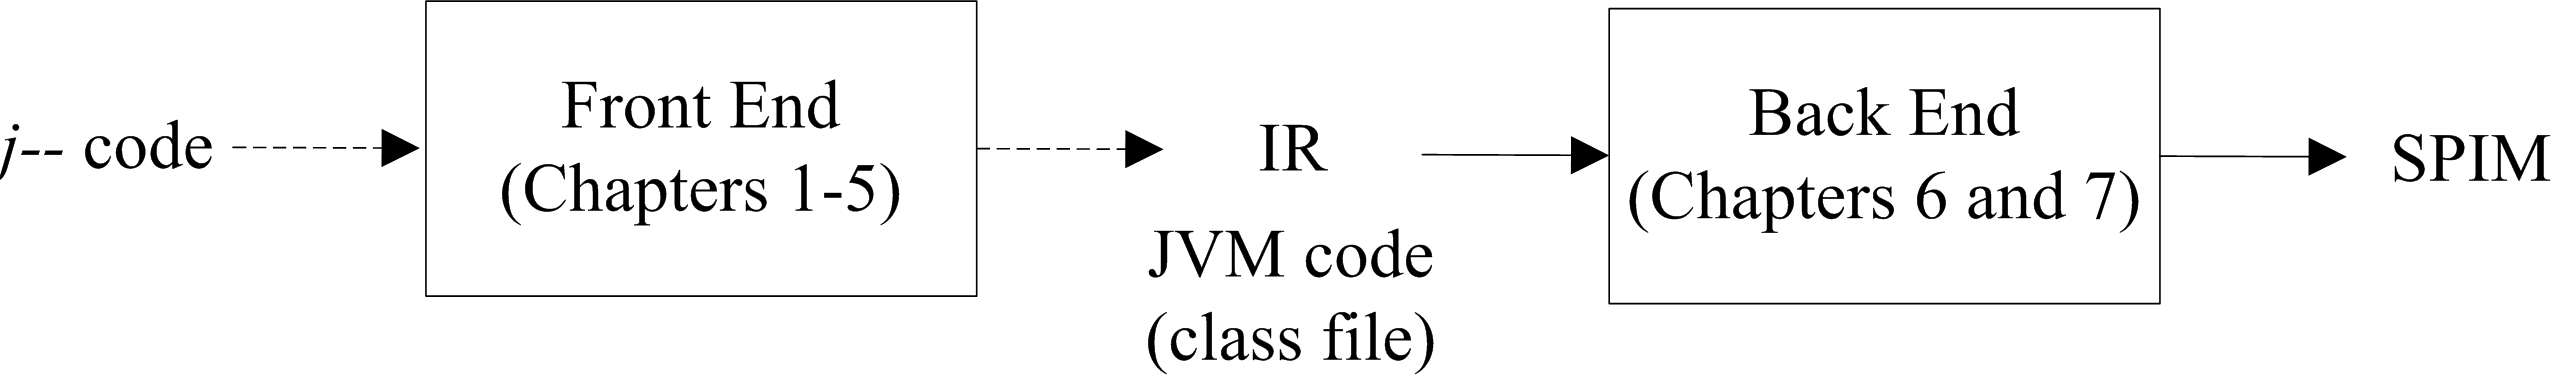
\includegraphics[scale=0.6]{{figures/figure06.01}.jpg}}
\end{center}

We re-define what constitute the IR, the front end and the back end
\begin{itemize}
\item JVM code is our new IR
\item The \jmm to JVM translator (Chapters 1 --- 5) is our new front end
\item The JVM to SPIM translator (Chapters 6 and 7) is our new back end
\end{itemize}

\pause
\bigskip

We translate enough JVM code to SPIM code to handle the \jmm program shown in the following slide
\end{frame}

\begin{frame}[fragile]
\pause

\begin{lstlisting}[language=Java]
import spim.SPIM;

// Prints factorial of a number computed using recursive and iterative
// algorithms.
public class Factorial {
    // Return the factorial of the given number computed recursively.
    public static int computeRec(int n) {
        if (n <= 0) {
            return 1;
        } else {
            return n * computeRec(n - 1);
        }
    }

    // Return the factorial of the given number computed iteratively.
    public static int computeIter(int n) {
        int result = 1;
        while ( n > 0 ) {
            result = result * n--;
	}
        return result;
    }

    // Entry point; print factorial of a number computed using
    // recursive and iterative algorithms.
    public static void main(String[] args) {
        int n = 7;
        SPIM.printInt(Factorial.computeRec(n));
	SPIM.printChar('\n');
        SPIM.printInt(Factorial.computeIter(n));
        SPIM.printChar('\n');
    }
}
\end{lstlisting}
\end{frame}

\begin{frame}[fragile]
\pause

We handle static methods, conditional statements, while loops, recursive method invocations, and enough arithmetic to do a few computations

\pause
\bigskip

We must deal with some objects, for example, constant strings

\pause
\bigskip

The program above refers to an array, but doesn't do anything with it so we do not implement array objects

\pause
\bigskip

So, our run-time support is minimal

\pause
\bigskip

To determine what JVM instructions must be handled, it is worth looking at the output from running \lstinline{javap} on \lstinline{Factorial.class}

\pause
\bigskip

\begin{lstlisting}[language={}]
public class Factorial extends java.lang.Object
  minor version: 0
  major version: 49
  Constant pool:
... <the constant pool is elided here> ...

{
public Factorial();
  Code:
   Stack=1, Locals=1, Args_size=1
   0: aload_0
   1: invokespecial #8; //Method java/lang/Object."<init>":()V
   4: return
\end{lstlisting}
\end{frame}

\begin{frame}[fragile]
\pause

\begin{lstlisting}[language={}]

public static int computeRec(int);
  Code:
   Stack=3, Locals=1, Args_size=1
   0: iload_0
   1: iconst_0
   2: if_icmpgt 10
   5: iconst_1
   6: ireturn
   7: goto  19
   10: iload_0
   11: iload_0
   12: iconst_1
   13: isub
   14: invokestatic #13; //Method computeRec:(I)I
   17: imul
   18: ireturn
   19: nop

public static int computeIter(int);
  Code:
   Stack=2, Locals=2, Args_size=1
   0: iconst_1
   1: istore_1
   2: iload_0
   3: iconst_0
   4: if_icmple 17
   7: iload_1
   8: iload_0
   9: iinc  0, -1
   12: imul
   13: istore_1
   14: goto 2
   17: iload_1
   18: ireturn
\end{lstlisting}
\end{frame}

\begin{frame}[fragile]
\pause

\begin{lstlisting}[language={}]

public static void main(java.lang.String[]);
  Code:
   Stack=1, Locals=2, Args_size=1
   0: bipush    7
   2: istore_1
   3: iload_1
   4: invokestatic  #13; //Method computeRec:(I)I
   7: invokestatic  #22; //Method spim/SPIM.printInt:(I)V
   10: bipush   10
   12: invokestatic #26; //Method spim/SPIM.printChar:(C)V
   15: iload_1
   16: invokestatic #28; //Method computeIter:(I)I
   19: invokestatic #22; //Method spim/SPIM.printInt:(I)V
   22: bipush   10
   24: invokestatic #26; //Method spim/SPIM.printChar:(C)V
   27: return
}
\end{lstlisting}
\end{frame}

\section{SPIM and the MIPS Architecture}
\begin{frame}[fragile]
\pause

The MIPS computer organization is shown below
\begin{center}
\visible<2->{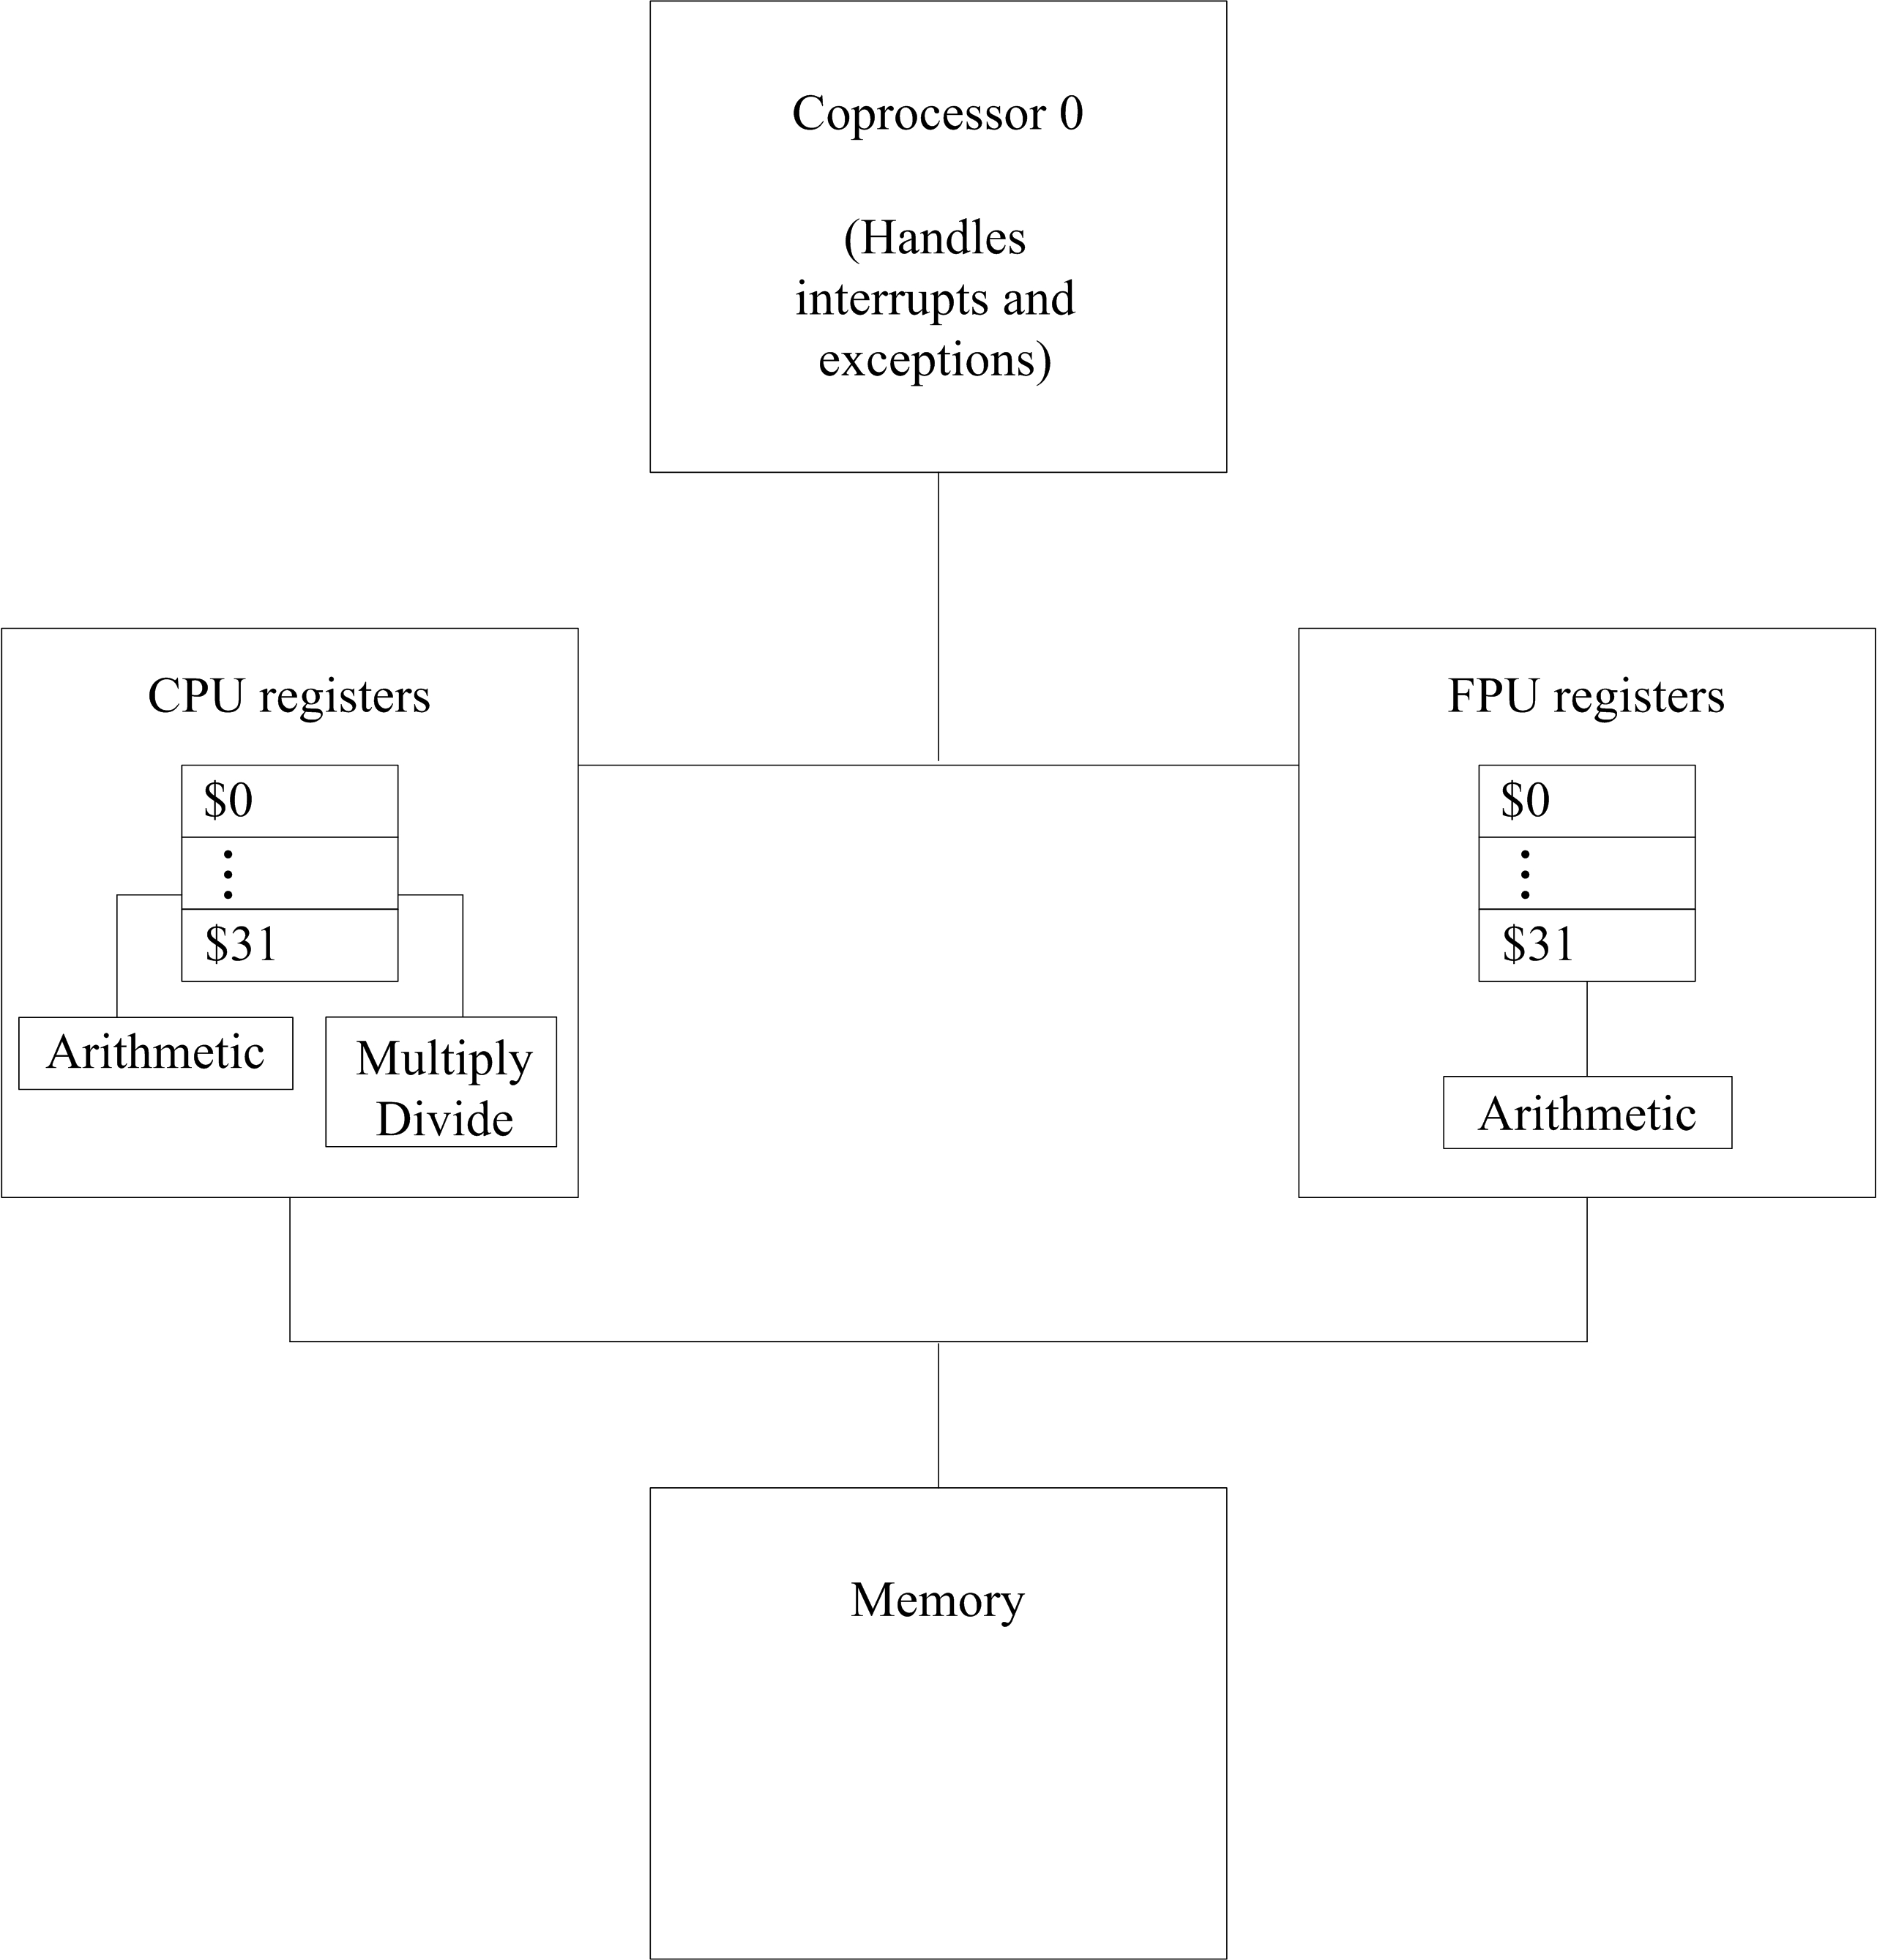
\includegraphics[scale=0.6]{{figures/figure06.02}.jpg}}
\end{center}
\end{frame}

\begin{frame}[fragile]
\pause

Memory organization, by convention divided into four segments, is shown below
\begin{center}
\visible<2->{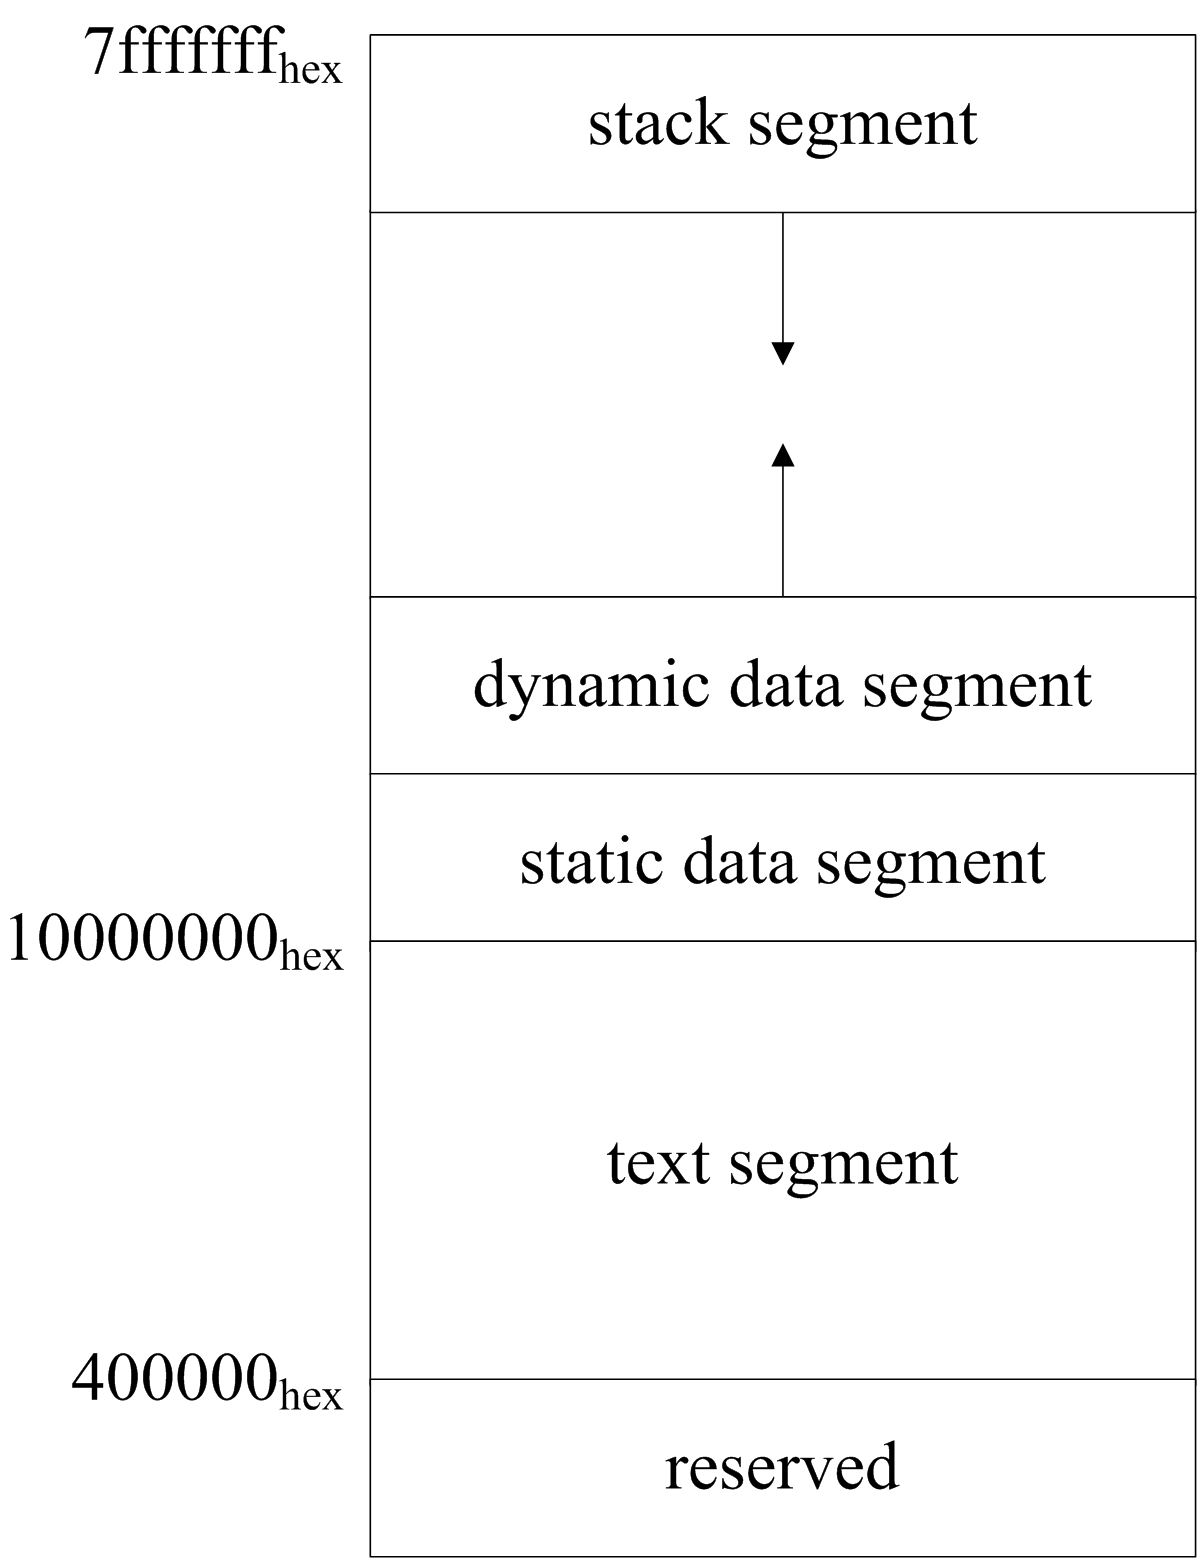
\includegraphics[scale=0.5]{{figures/figure06.03}.jpg}}
\end{center}

\begin{itemize}
\item Text segment - The program's instructions go here
\item Static data segment - Static data, which exist for the duration of the program, go here
\item Dynamic data segment (aka heap) - This is where objects and arrays are dynamically
allocated during execution of the program
\item Like the stack for the JVM, every time a routine is called, a new stack frame is pushed onto the stack; every time a return is executed, a frame is popped off
\end{itemize}
\end{frame}

\begin{frame}[fragile]
\pause

Many of the thirty two (0 -- 31) 32-bit general-purpose registers, by convention are designated for special uses, and have alternative names
\begin{itemize}
\item \$zero (0) always holds the constant 0
\item \$at (1)  is reserved for use by the assembler
\item \$v0 and \$v1 (2 and 3) are used for expression evaluation and as the results of a function
\item \$a0 -- \$a3 (4 -- 7) are used for passing the first four arguments to routines; any additional
arguments are passed on the stack
\item \$t0 -- \$t7 (8 -- 15) are meant to hold temporary values that need not be preserved across
routine calls; if they must be preserved, it is up to the caller to save them
\item \$s0 -- \$s7 (16 -- 23) are meant to hold values that must be preserved across routine calls; it is up to the callee to save these registers
\item \$t8 and \$t9 (24 and 25) are caller-saved temporaries
\item \$k0 and \$k1 (26 and 27) are reserved for use by the operating system kernel
\item \$gp (28) is a global pointer to the middle of a 64K block of memory in the static data segment
\item \$sp (29) is the stack pointer, pointing to the last location on the stack
\item \$fp (30) is the stack frame pointer, pointing to the latest frame on the stack
\item \$ra (31) is the return address register, holding the address to which execution should continue upon return from the latest routine
\end{itemize}
\end{frame}

\begin{frame}[fragile]
\pause

SPIM assumes we follow a particular protocol in implementing routine calls, when one
routine (the caller) invokes another routine (the callee)

\pause
\bigskip

Most bookkeeping for routine invocation is recorded in a stack frame on the run-time stack segment, as is done in the JVM; but here we must also deal with registers

\pause
\bigskip

The stack frame for an invoked routine is shown below
\begin{center}
\visible<4->{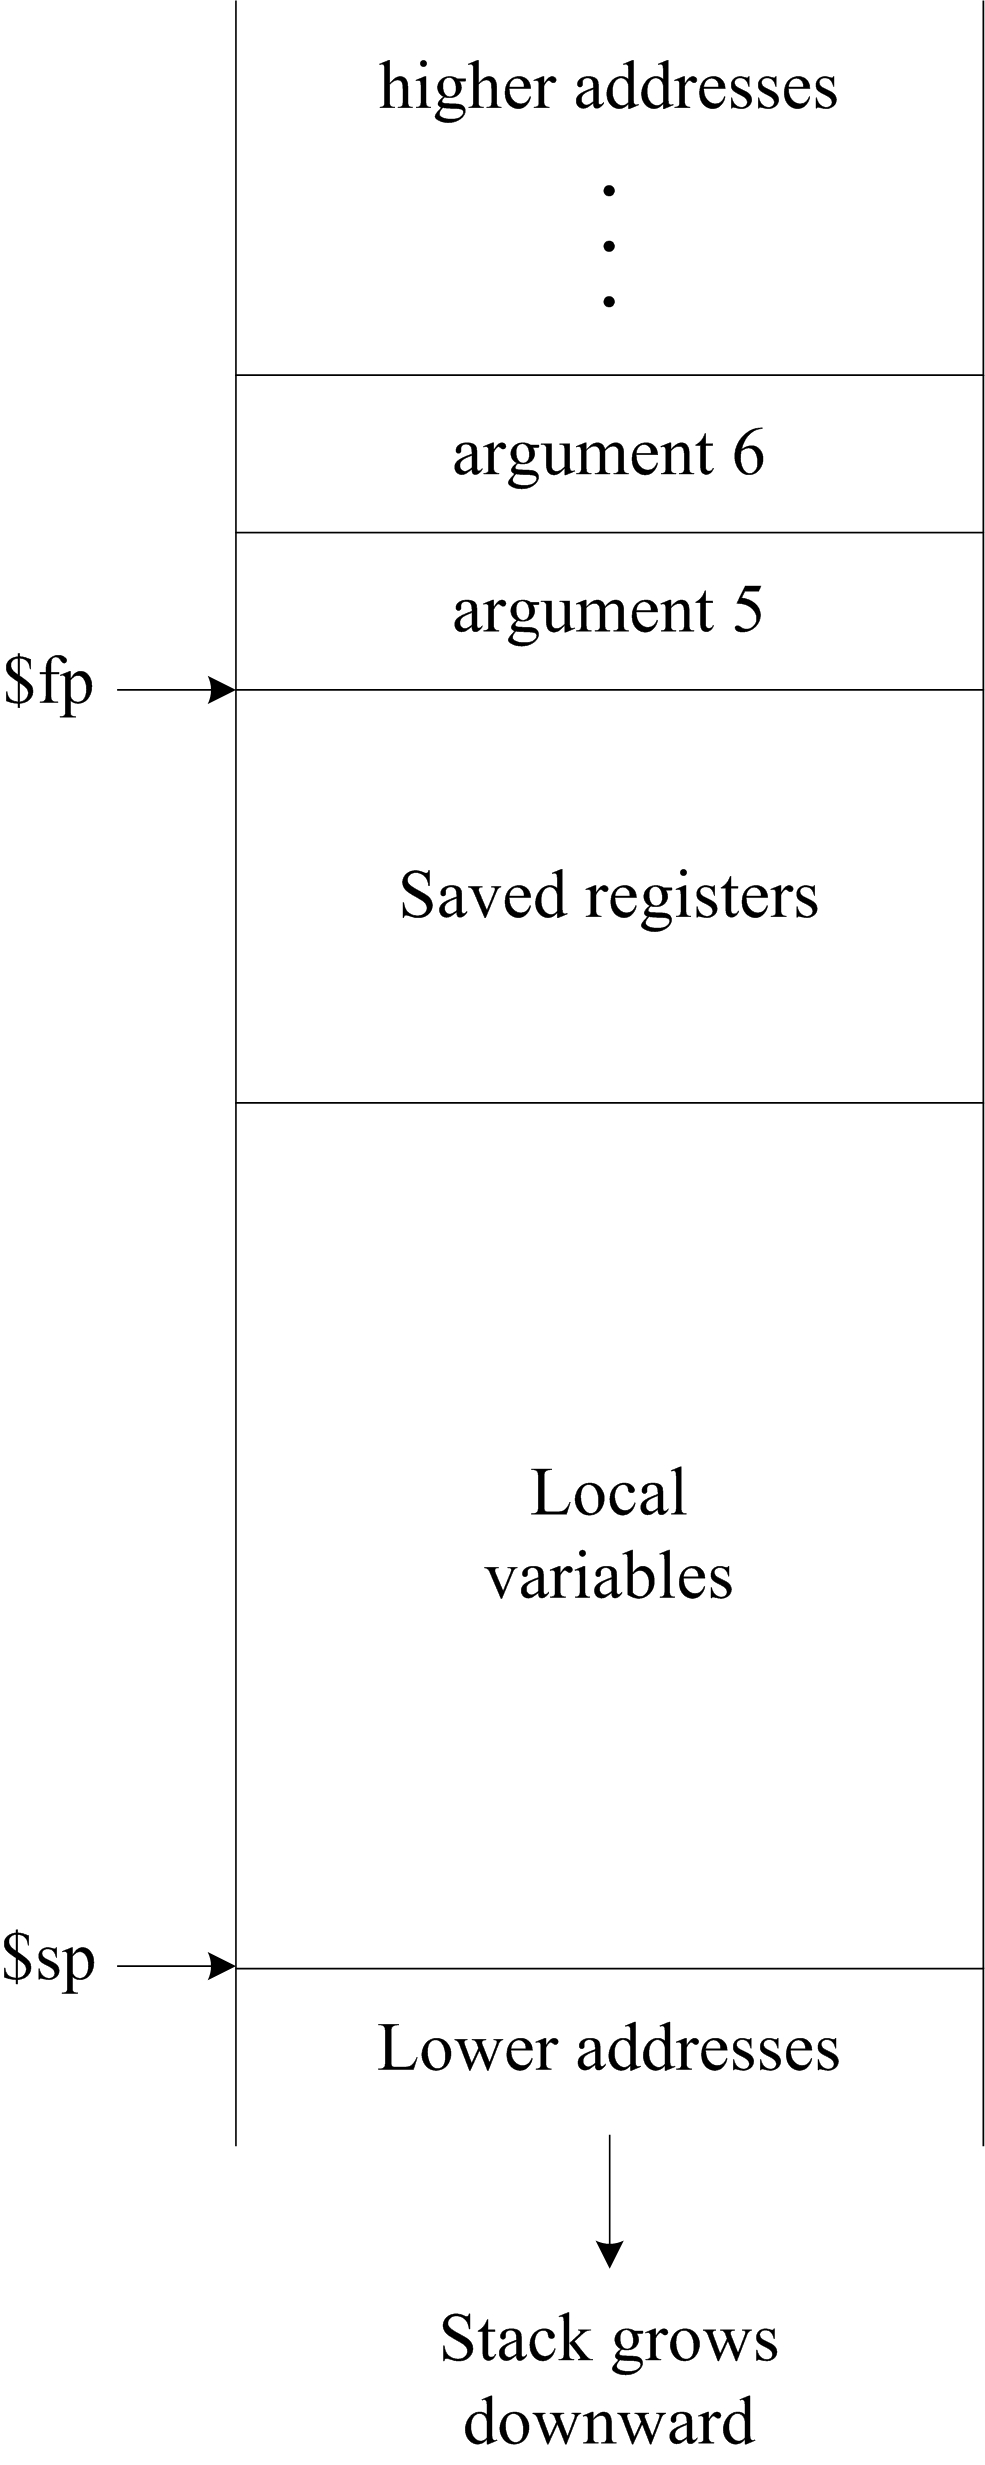
\includegraphics[scale=0.4]{{figures/figure06.04}.jpg}}
\end{center}

\pause
\bigskip

SPIM provides a set of system calls for accessing simple input and output functions
\end{frame}

\section{Our Translator}
\begin{frame}[fragile]
\pause

Phases of our JVM to SPIM translator are shown below
\begin{center}
\visible<2->{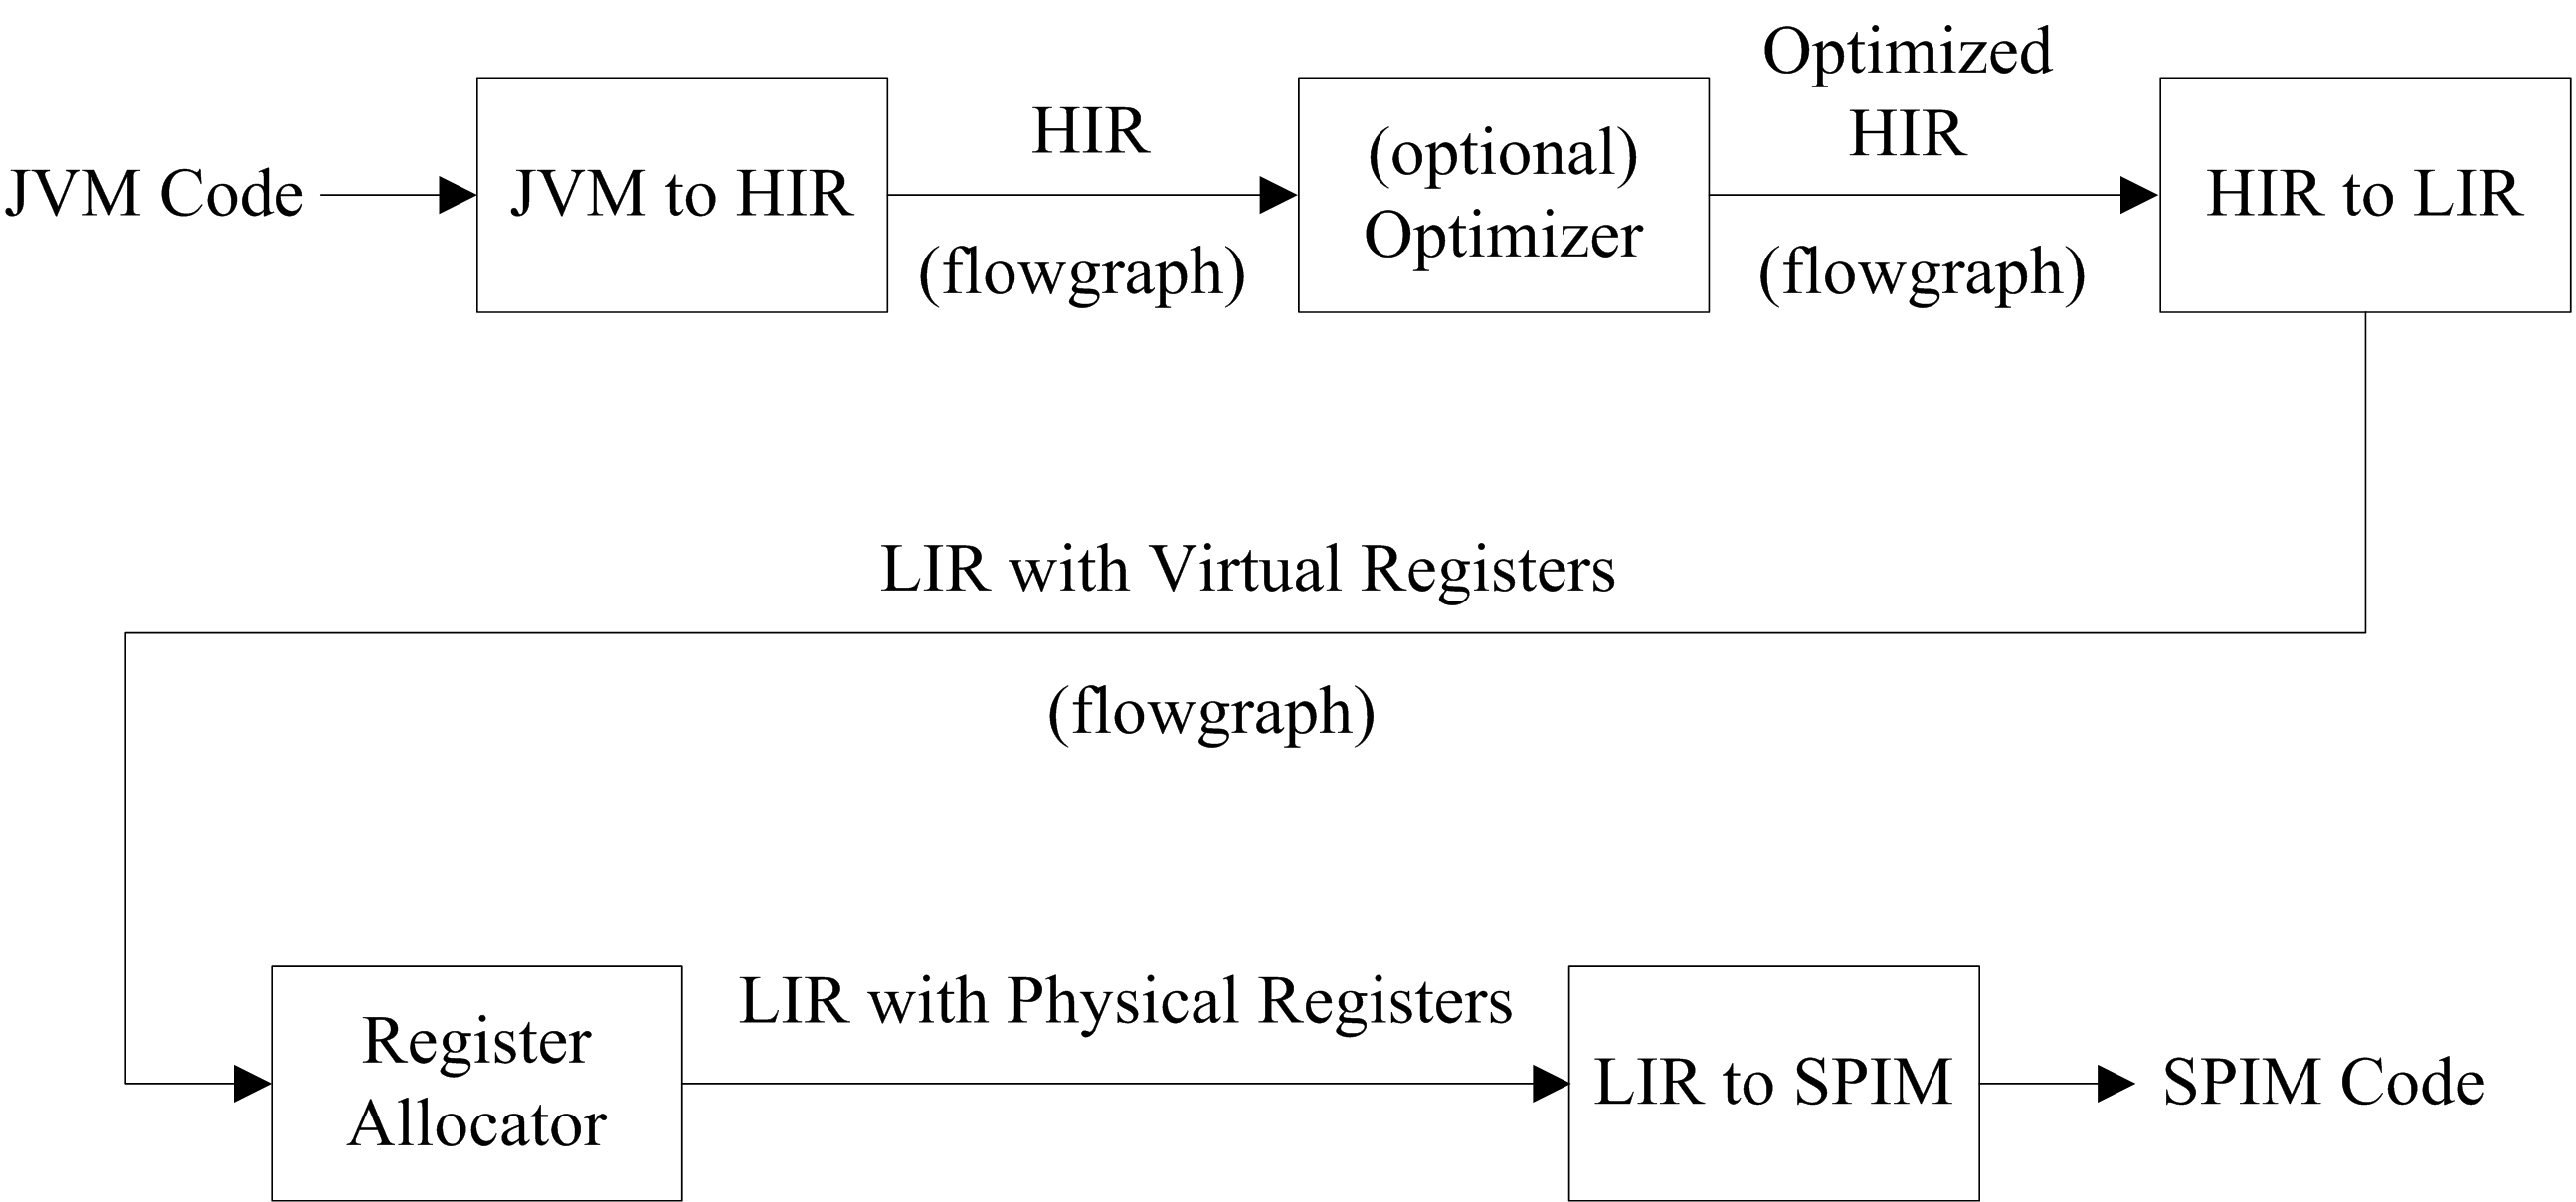
\includegraphics[scale=0.6]{{figures/figure06.06}.jpg}}
\end{center}

\pause
\bigskip

The first step is to scan through the JVM instructions and construct a flow graph of basic blocks

\pause
\bigskip

A basic block is a sequence of instructions with just one entry point at the start and one exit point at the end; otherwise, there are no branches into or out of the instruction sequence
\end{frame}

\begin{frame}[fragile]
\pause

Consider the \lstinline{computeIter()} method from our \lstinline{Factorial} example 
\begin{lstlisting}[language=Java]
    public static int computeIter(int n) {
        int result = 1;
        while ( n > 0 ) {
            result = result * n--;
        }
        return result;
    }
\end{lstlisting}

\pause
\bigskip

The JVM code for the method is shown below (line breaks to delineate basic blocks)
\begin{lstlisting}[language={}]
public static int computeIter(int);
  Code:
   Stack=2, Locals=2, Args_size=1

   0: const_1
   1: istore_1

   2: iload_0
   3: iconst_0
   4: if_icmple 17

   7: iload_1
   8: iload_0
   9: iinc  0, -1
   12: imul
   13: istore_1
   14: goto 2

   17: iload_1
   18: ireturn
\end{lstlisting}
\end{frame}

\begin{frame}[fragile]
\pause

The control-flow graph, expressed as a graph constructed from the basic blocks is shown below
\begin{center}
\visible<2->{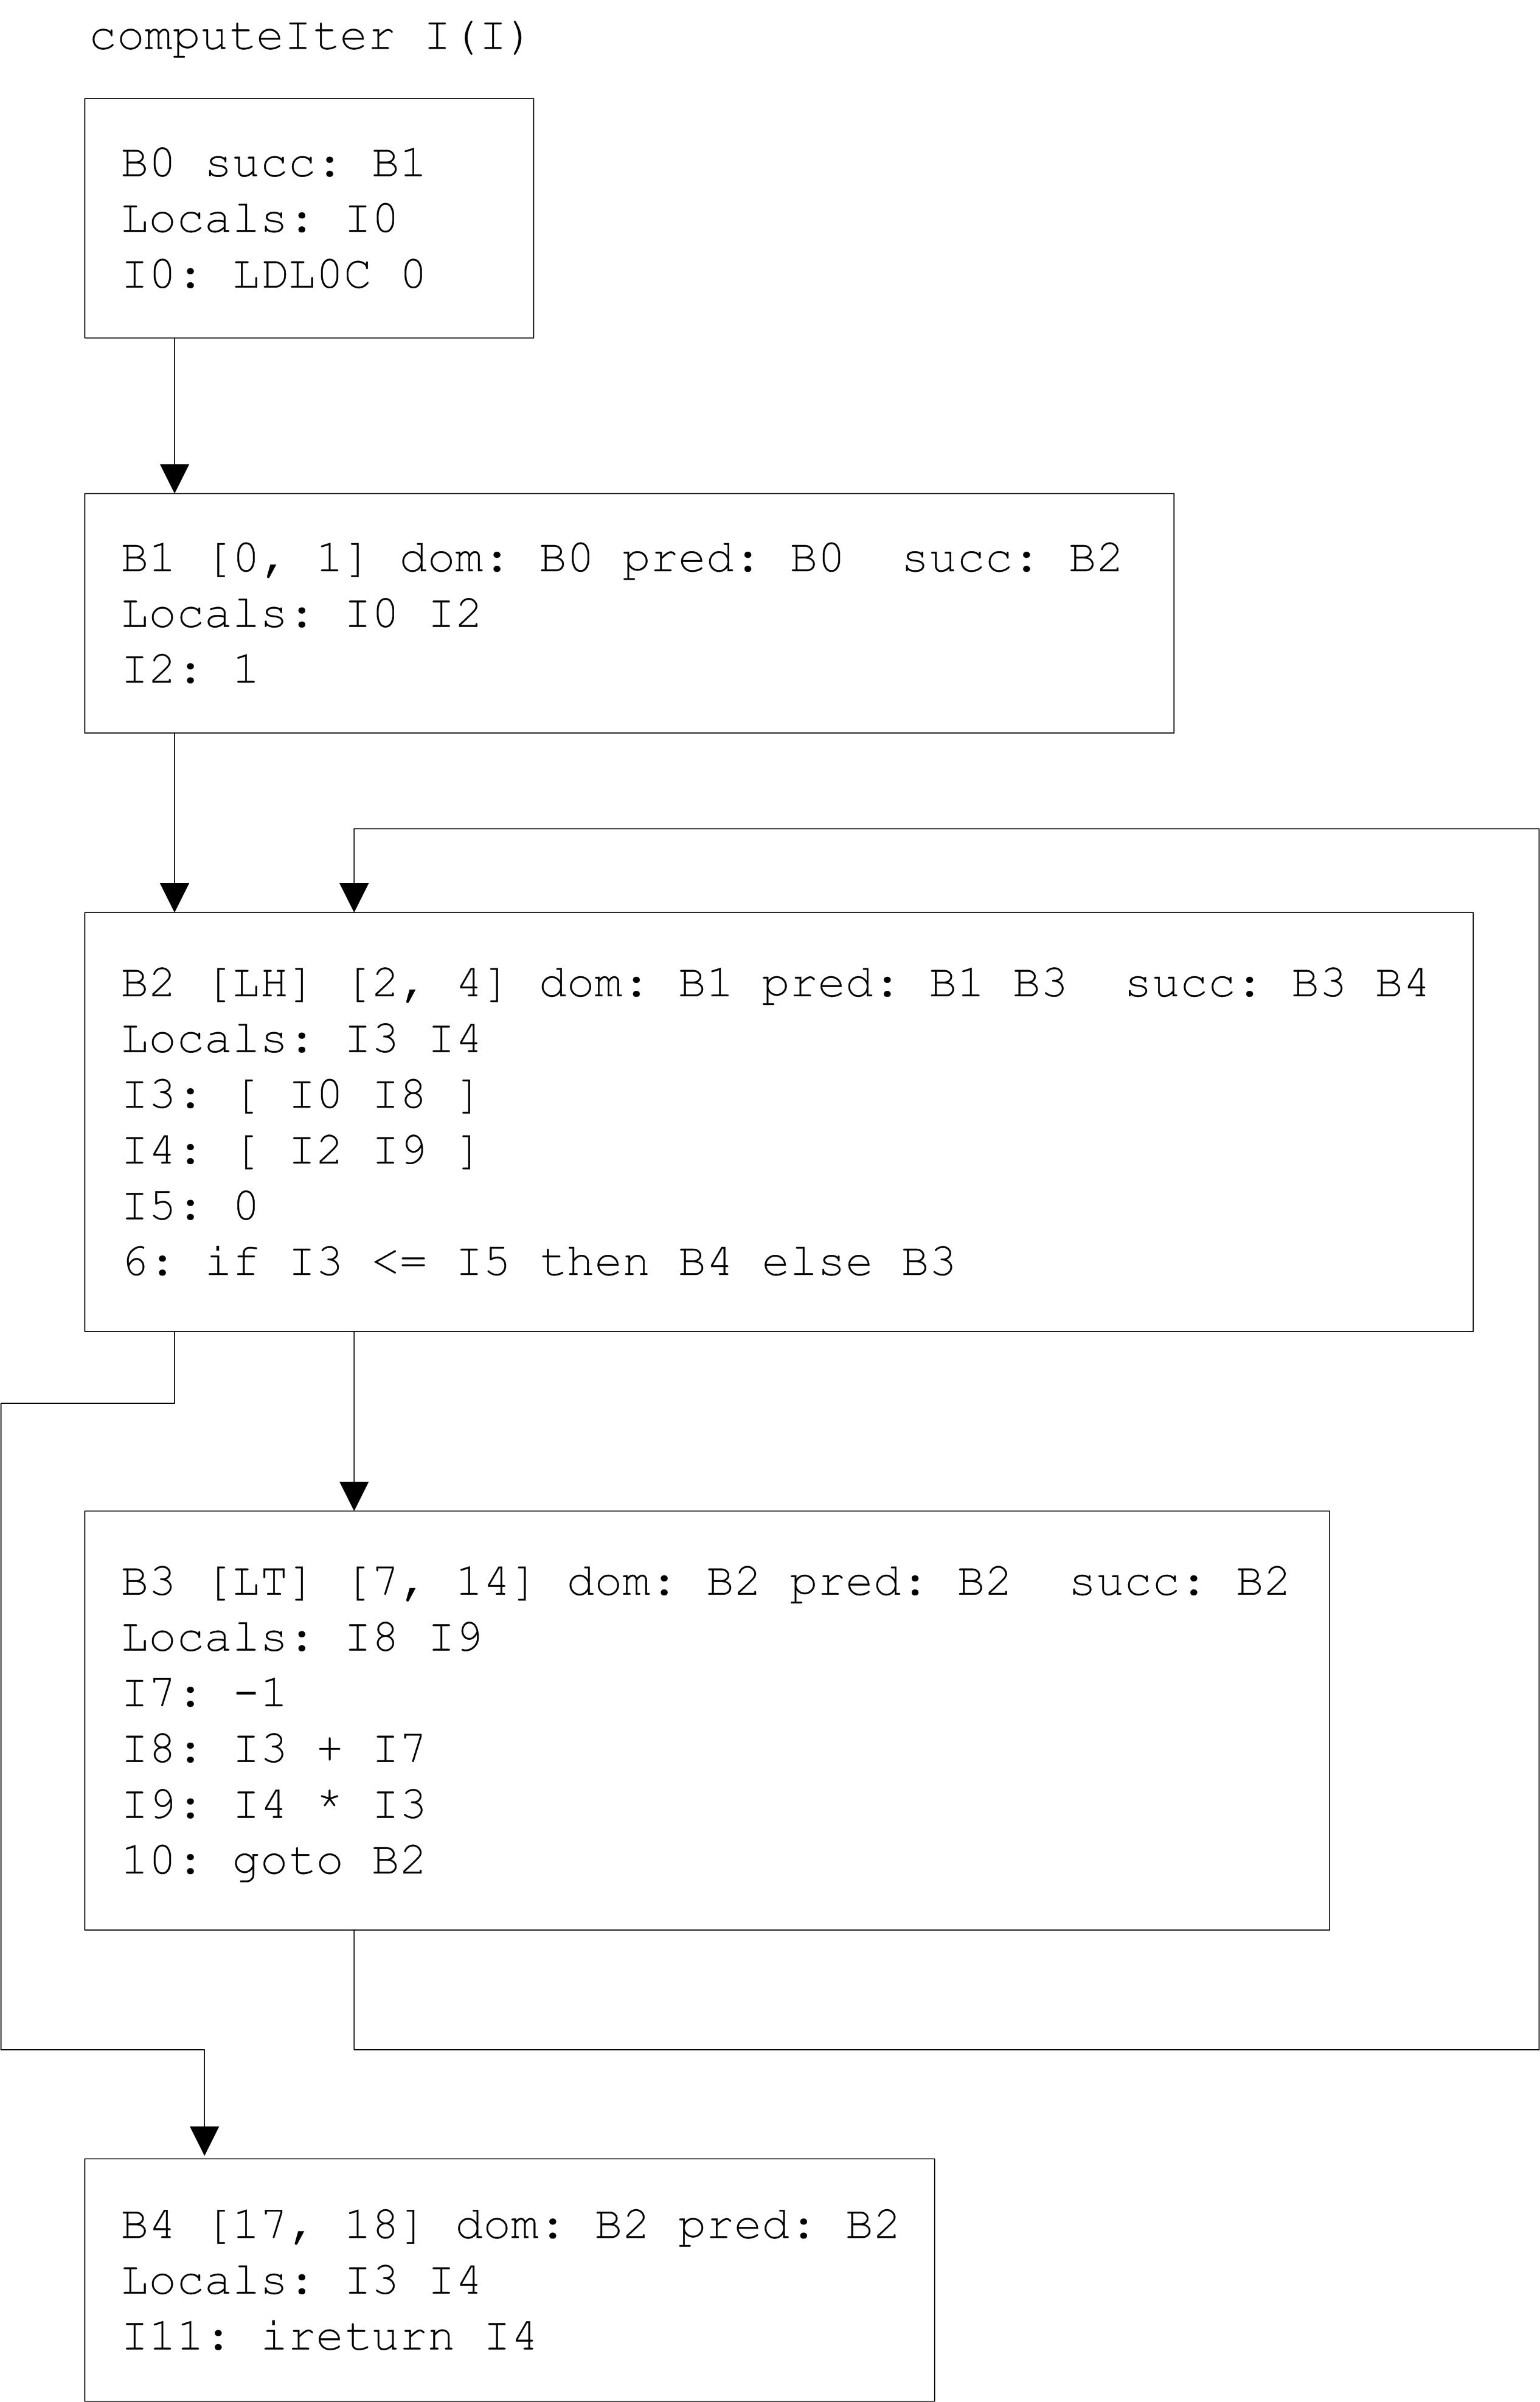
\includegraphics[scale=0.4]{{figures/figure06.07}.jpg}}
\end{center}
\end{frame}

\begin{frame}[fragile]
\pause

The boxes represent the basic blocks and the arrows indicate the flow of control among the blocks

\pause
\bigskip

The first line of text within each box identifies the block, a list of any successor blocks (labeled by \lstinline{succ}) and a list of any predecessor blocks (labeled by \lstinline{pred})

\pause
\bigskip

We add an extra beginning block \lstinline{B0} for the method's entry point

\pause
\bigskip

The denotation \lstinline{[LH]} on the first line of \lstinline{B2} indicates that \lstinline{B2} is a loop header

\pause
\bigskip

The denotation \lstinline{[LT]} on the first line of \lstinline{B3} indicates that \lstinline{B3} is a loop tail

\pause
\bigskip

The pairs of numbers within square brackets, for example \lstinline{[7, 14]} on the first line of \lstinline{B3}, denote the ranges of JVM instructions captured in the block

\pause
\bigskip

The denotation \lstinline{dom} labels the basic block's immediate dominator

\pause
\bigskip

A node $d$ is said to dominate a node $n$ if every path from the entry node (\lstinline{B0}) to $n$ must go through $d$

\pause
\bigskip

A node $d$ strictly dominates $n$ if it dominates $n$ but is not the same as $n$

\pause
\bigskip

Node $d$ is an immediate dominator of node $n$ if $d$ strictly dominates $n$ but does not dominate any other node that strictly dominates $n$, ie, it is the node on the path from the entry node to $n$ that is the ``closest'' to $n$
\end{frame}

\begin{frame}[fragile]
\pause

Local variables are tracked in a state vector called \lstinline{Locals} and are indexed in this vector
by their location in the JVM stack frame

\pause
\bigskip

The current state of this vector at the end of a block's instruction sequence is printed on the block's second line and labeled with \lstinline{Locals}

\pause
\bigskip

The values are listed in positional order and each value is represented by the instruction ID for the instruction that computes it

\pause
\bigskip

For example, in \lstinline{B0} this vector has just one element, corresponding to the method's formal argument \lstinline{n}; in \lstinline{B1} the vector has two elements: the first is \lstinline{I0} for \lstinline{n} and the second is \lstinline{I2} for result

\pause
\bigskip

The instruction sequence within each basic block is of a higher level than is JVM code

\pause
\bigskip

For example, the \jmm statement 
\begin{lstlisting}[language=Java]
w = x + y + z;
\end{lstlisting}
\noindent might bre represented in HIR by
\begin{lstlisting}[language={}]
I8: I0 + I1
I9: I8 + I2
\end{lstlisting}
where \lstinline{I0}, \lstinline{I1} and \lstinline{I2} refer to the instruction IDs labeling instructions that compute values for \lstinline{x}, \lstinline{y} and \lstinline{z} respectively
\end{frame}

\begin{frame}[fragile]
\pause

The instruction for loading a constant is simply the constant itself; for example, the single instruction from block \lstinline{B1} 
\begin{lstlisting}[language={}]
I2: 1
\end{lstlisting}

\pause
\bigskip

Not all instructions generate values; for example, the instruction
\begin{lstlisting}[language={}]
6: if I3 <= I5 then B4 else B3
\end{lstlisting}
\noindent in block \lstinline{B2} produces no value but transfers control to either \lstinline{B4} or \lstinline{B3}
\end{frame}

\begin{frame}[fragile]
\pause

Our HIR employs static single assignment (SSA) form, where for every variable, there is just one place in the method where that variable is assigned a value, which means that when a variable is re-assigned in the method, one must create a new version for it

\pause
\bigskip

For example, given the simple sequence
\begin{lstlisting}[language=Java]
x = 3;
x = x + y;
\end{lstlisting}
we might subscript our variables to distinguish different versions
\begin{production}
\subs{\text{\lstinline{x}}}{\text{1}} \lstinline{= 3;}
\subs{\text{\lstinline{x}}}{\text{2}} \lstinline{=} \subs{\text{\lstinline{x}}}{\text{1}} \lstinline{+} \subs{\text{\lstinline{y}}}{\text{1}}\lstinline{;}
\end{production}

\pause
\bigskip

In the HIR we represent a variable's value by the instruction that computed it and we track these values in the state vector

\pause
\bigskip

The value in a state vector's element may change as we sequence through the block's instructions

\pause
\bigskip

If the next block has just one predecessor, it can copy the predecessor's state vector at its start; if there are two or more predecessors, the states must be merged
\end{frame}

\begin{frame}[fragile]
\pause

For example, consider the following \jmm method, where the variables are in SSA form.
\begin{production}
\lstinline{static int ssa(int} \subs{\text{\lstinline{w}}}{\text{1}}\lstinline{) \{}
    \lstinline{if (}\subs{\text{\lstinline{w}}}{\text{1}} \lstinline{\> 0) \{}
        \subs{\text{\lstinline{w}}}{\text{2}} \lstinline{= 1;}
    \lstinline{\}}
    \lstinline{else \{}
        \subs{\text{\lstinline{w}}}{\text{3}} \lstinline{= 2;}
    \lstinline{\}}
    \lstinline{return} \subs{\text{\lstinline{w}}}{\text{?}}\lstinline{;}
\lstinline{\}}
\end{production}

\pause
\bigskip

In the statement 
\begin{production}
\lstinline{return} \subs{\text{\lstinline{w}}}{\text{?}}\lstinline{;}
\end{production}
which \lstinline{w} do we return?

\pause
\bigskip

We solve this problem by using what is called a Phi function, a special HIR instruction that captures the possibility of a variable having one of several values; in our example, the final block would contain the following code
\begin{production}
\subs{\text{\lstinline{w}}}{\text{4}} = [\subs{\text{\lstinline{w}}}{\text{2}}  \subs{\text{\lstinline{w}}}{\text{3}}];
\lstinline{return} \subs{\text{\lstinline{w}}}{\text{4}}\lstinline{;}
\end{production}
\end{frame}

\begin{frame}[fragile]
\pause

Another place where Phi functions are needed are in loop headers, basic blocks having at least one incoming backward branch and at least two predecessors, as illustrated below

\begin{center}
\visible<2->{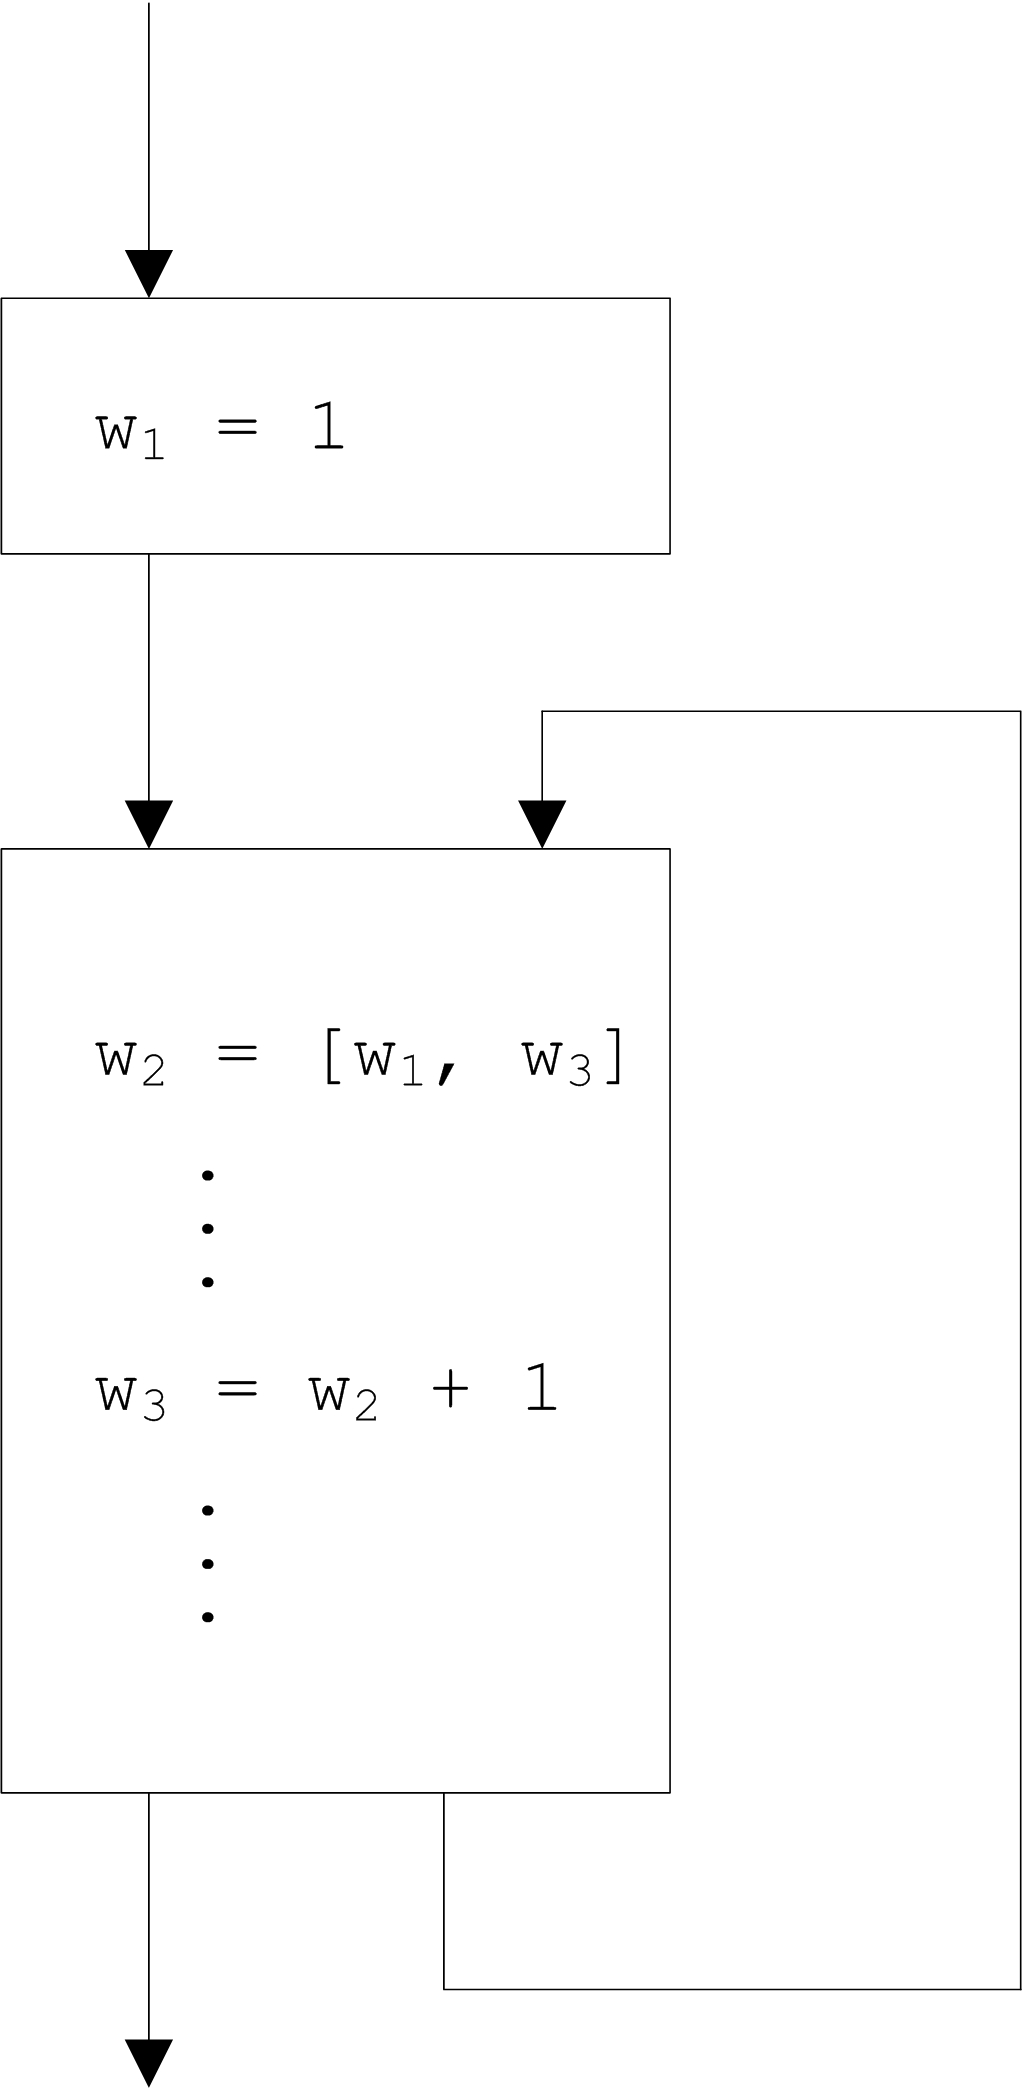
\includegraphics[scale=0.5]{{figures/figure06.11}.jpg}}
\end{center}
\end{frame}

\begin{frame}[fragile]
\pause

We conservatively define Phi functions for all variables and then remove redundant Phi functions later

\pause
\bigskip

In the first instance, $\text{\lstinline{w}}_2$ can be defined as a Phi function with operands $\text{\lstinline{w}}_1$  and $\text{\lstinline{w}}_2$
\begin{production}
\subs{\text{\lstinline{w}}}{\text{2}}  = [\subs{\text{\lstinline{w}}}{\text{1}} \subs{\text{\lstinline{w}}}{\text{2}}]
\end{production}

\pause
\bigskip

When \lstinline{w} is later incremented, the second operand may be overwritten by the new $\text{\lstinline{w}}_3$
\begin{production}
\subs{\text{\lstinline{w}}}{\text{2}} = [\subs{\text{\lstinline{w}}}{\text{1}} \subs{\text{\lstinline{w}}}{\text{3}}]
\end{production}

\pause

A redundant Phi function will not be changed and can be removed

\pause
\bigskip

If the \lstinline{w} is never modified in the loop body, the Phi function instruction takes the form
\begin{production}
\subs{\text{\lstinline{w}}}{\text{2}} = [\subs{\text{\lstinline{w}}}{\text{1}} \subs{\text{\lstinline{w}}}{\text{2}}]
\end{production}

\pause
\bigskip

Phi functions are tightly bound to state vectors, so when a block is processed
\begin{itemize}
\item If the block has just a single predecessor, then it may inherit the state vector of that predecessor; the states are simply copied
\item If the block has more than one predecessor, then those states in the vectors that differ must be merged using Phi functions
\item For loop headers we conservatively create Phi functions for all variables, and then later remove redundant Phi functions
\end{itemize}
\end{frame}

\begin{frame}[fragile]
\pause

The translation process from JVM instructions to HIR takes place in the constructor \lstinline{NEmitter()} in the class \lstinline{NEmitter}; for each method, the control-flow graph HIR is constructed in several steps

\pause
\bigskip

The \lstinline{NControlFlowGraph} constructor is invoked on the method, which produces the control-flow graph \lstinline{cfg}; in this first step, the JVM code is translated to sequences of tuples

\begin{enumerate}
\item Objects of type \lstinline{NBasicBlock} represent the basic blocks in the control-flow graph; the control flow is captured by the links, \lstinline{successors} in each block; there are also the links \lstinline{predecessors} for analysis

\item The JVM code is first translated to a list of tuples, corresponding to the JVM instructions; each block stores its sequence of tuples in an \lstinline{ArrayList} called \lstinline{tuples}
\end{enumerate}

\pause
\bigskip

The method call
\begin{lstlisting}[language=Java]
cfg.detectLoops(cfg.basicBlocks.get(0), null);
\end{lstlisting}
detects loop headers and loop tails

\pause
\bigskip

The method call
\begin{lstlisting}[language=Java]
cfg.removeUnreachableBlocks();
\end{lstlisting}
removes unreachable blocks
\end{frame}

\begin{frame}[fragile]
\pause

The method call
\begin{lstlisting}[language=Java]
cfg.computeDominators(cfg.basicBlocks.get(0), null);
\end{lstlisting}
computes an immediate dominator for each basic block, that closest predecessor through which all paths must pass to reach the target block; it's a useful place to which insert invariant code that is lifted out of a loop in optimization

\pause
\bigskip

The method call
\begin{lstlisting}[language=Java]
cfg.tuplesToHir();
\end{lstlisting}
converts the tuples representation to HIR, stored as a sequence of HIR instructions in the array list \lstinline{hir} for each block

\pause
\bigskip

The method call
\begin{lstlisting}[language=Java]
cfg.eliminateRedundantPhiFunctions();
\end{lstlisting}
eliminates unnecessary Phi functions and replaces them with their simpler values

\pause
\bigskip

The HIR is now ready for further analysis
\end{frame}

\begin{frame}[fragile]
\pause

That the HIR is in SSA form makes it amenable to several simple optimizations, which make for fewer instructions and/or faster programs

\pause
\bigskip

Local optimizations are improvements made based on analysis of the linear sequence of instructions within a basic block

\pause
\bigskip

Global optimizations require an analysis of the whole control graph and involve what is called data-flow analysis

\pause
\bigskip

In some cases, the code of a callee's body can replace the call sequence in the caller's code, saving the overhead of a routine call --- we call this inlining; for example, consider the following code

\begin{lstlisting}[language=Java]
static int getA() {
    return Getter.a;
}

static void foo() {
    int i;
    i = getA();
}
\end{lstlisting}

can be replaced with

\begin{lstlisting}[language=Java]
static void foo() {
    int i;
    i = Getter.a;
}
\end{lstlisting}
\end{frame}

\begin{frame}[fragile]
\pause

Expressions having operands that are both constants, or variables whose values are known to be constants, can be folded, that is replaced by their constant value

\pause
\bigskip

For example, consider the Java method

\begin{lstlisting}[language=Java]
static void foo() {
    int i = 1;
    int j = 2;
    int k = i + j + 3;
}
\end{lstlisting}

and the corresponding HIR code

\begin{lstlisting}[language={}]
  B0 succ: B1
  Locals:
    0: 0
    1: 1
    2: 2

  B1 [0, 10] dom: B0 pred: B0
  Locals:
    0: I3
    1: I4
    2: I7
  I3: 1
  I4: 2
  I5: I3 + I4
  I6: 3
  I7: I5 + I6
  8: return
\end{lstlisting}

\pause
\bigskip

The instruction \lstinline{I3 + I4} at \lstinline{I5} can be replaced by the constant \lstinline{3} and the \lstinline{I5 + I6} at \lstinline{I7} can replaced by the constant \lstinline{6}
\end{frame}

\begin{frame}[fragile]
\pause

Another optimization one may make is common subexpression elimination, where we identify expressions that are re-evaluated even if their operands are unchanged; for example, in the following method

\begin{lstlisting}[language=Java]
void foo(int i) {
    int j = i * i * i;
    int k = i * i * i;
}
\end{lstlisting}

we can replace

\begin{lstlisting}[language=Java]
int k = i * i * i;
\end{lstlisting}

in \lstinline{foo()} with the more efficient

\begin{lstlisting}[language=Java]
int k = j;
\end{lstlisting}

\pause
\bigskip

Common subexpressions do arise in places one might not expect them; for example, consider the following C language fragment
\begin{lstlisting}[language=C]
for (i = 0; i < 1000; i++) {
    for (j = 0; j < 1000; j++) {
        c[i][j] = a[i][j] + b[i][j];
    }
}
\end{lstlisting}
where \lstinline{a}, \lstinline{b}, and \lstinline{c} are integer matrices 

\pause
\bigskip

If \lstinline{a'}, \lstinline{b'}, and \lstinline{c'} are their base addresses respectively, then the memory addresses of \lstinline{a[i][j]}, \lstinline{b[i][j]}, and \lstinline{c[i][j]} are \lstinline{a' + i * 4 * 1000 + j * 4}, \lstinline{b' + i * 4 * 1000 + j * 4}, and \lstinline{c' + i * 4 * 1000 + j * 4}; eliminating the common offsets, \lstinline{i * 4 * 1000 + j * 4}, can save us a lot of computation
\end{frame}

\begin{frame}[fragile]
\pause

Loop invariant expressions can be lifted out of the loop and computed in the predecessor block to the loop header

\pause
\bigskip

For example, the following \jmm code for summing two matrices
\begin{lstlisting}[language=Java]
int i = 0;
while (i <= 999) {
    int j = 0;
    while (j <= 999) {
        c[i][j] = a[i][j] + b[i][j];
        j = j + 1;;
    }
    i = i + 1;
}
\end{lstlisting}

can be rewritten as 

\begin{lstlisting}[language=Java]
int i = 0;
while (i <= 999) {
    int[] ai = a[i];
    int[] bi = b[i];
    int[] ci = c[i];
    int j = 0;
    while (j <= 999)
    {
        ci[j] = ai[j] + bi[j];
        j = j + 1;;
    }
    i = i + 1;
}
\end{lstlisting}
\end{frame}

\begin{frame}[fragile]
\pause

When indexing an array, we must check that the index is within bounds; for example, in our code for matrix addition, in the assignment

\begin{lstlisting}[language=Java]
c[i][j] = a[i][j] + b[i][j];
\end{lstlisting}
\noindent the \lstinline{i} and \lstinline{j} must be tested to make sure each is greater than or equal to zero, and less than 1000; and this must be done for each of \lstinline{c}, \lstinline{a} and \lstinline{b}

\pause
\bigskip

But if we know that \lstinline{a}, \lstinline{b} and \lstinline{c} are all of like dimensions, then once the check is done for \lstinline{a}, it need not be repeated for \lstinline{b} and \lstinline{c}

\pause
\bigskip

Every time we send a message to an object, or access a field of an object, we must insure that the object is not the special null object; for example, in
\begin{lstlisting}[language=Java]
...a.f...
\end{lstlisting}
we want to make sure that \lstinline{a} is non-null before computing the offset to the field \lstinline{f}

\pause
\bigskip

But we may know that \lstinline{a} is non-null; for example, in the following code
\begin{lstlisting}[language=Java]
...a.f...
...a.g...
...a.h...
\end{lstlisting}
once we've done the null-check for \lstinline{a.f} there is no reason to do it again for either \lstinline{a.g} or \lstinline{a.h}

\pause
\bigskip

The HIR does not present every opportunity for optimization, particularly those involving
back branches (in loops); for this we would need full data-flow analysis where we compute where in the code computed values remain valid
\end{frame}

\begin{frame}[fragile]
\pause

Since the HIR is not necessarily suitable for register allocation, we translate it into a low-level intermediate representation (LIR) where

\begin{itemize}
\item Phi functions are removed from the code and replaced by explicit moves

\item Instruction operands are expressed as explicit virtual registers
\end{itemize}

\pause
\bigskip

For example, the LIR for \lstinline{Factorial.computeIter()} is shown below

\begin{lstlisting}[language={}]
computeIter (I)I

  B0

  B1
  0: LDC [1] [V32|I]
  5: MOVE $a0 [V33|I]                                                                                                                                                                                                                         
  10: MOVE [V32|I] [V34|I]                                                                                                                                                                                                                    
                                                                                                                                                                                                                                              
  B2                                                                                                                                                                                                                                          
  15: LDC [0] [V35|I]                                                                                                                                                                                                                         
  20: BRANCH [LE] [V33|I] [V35|I] B4                                                                                                                                                                                                          
                                                                                                                                                                                                                                              
  B3                                                                                                                                                                                                                                          
  25: LDC [-1] [V36|I]                                                                                                                                                                                                                        
  30: ADD [V33|I] [V36|I] [V37|I]                                                                                                                                                                                                             
  35: MUL [V34|I] [V33|I] [V38|I]                                                                                                                                                                                                             
  40: MOVE [V38|I] [V34|I]                                                                                                                                                                                                                    
  45: MOVE [V37|I] [V33|I]                                                                                                                                                                                                                    
  50: BRANCH B2                                                                                                                                                                                                                               
                                                                                                                                                                                                                                              
  B4                                                                                                                                                                                                                                          
  55: MOVE [V34|I] $v0
  60: RETURN $v0
\end{lstlisting}
\end{frame}

\begin{frame}[fragile]
\pause

In the above example, seven virtual registers \lstinline{V32} -- \lstinline{V38} are allocated to the LIR computation

\pause
\bigskip

Two physical registers, \lstinline{$a0} for the argument \lstinline{n} and \lstinline{$v0} for the return value, are referred to by their symbolic names

\pause
\bigskip

We start enumerating virtual registers beginning at 32; the numbers 0 through 31 are reserved for enumerating physical registers

\pause
\bigskip

LIR instructions are read from left to right

\pause
\bigskip

We enumerate the LIR instructions by multiples of five, which eases the insertion of spill (and restore) instructions, which may be required for register allocation
\end{frame}

\begin{frame}[fragile]
\pause

The process of translating HIR to LIR is relatively straightforward and is a two-step
process
\begin{enumerate}
\item The \lstinline{NEmitter} constructor invokes the \lstinline{NControlFlowGraph} method \lstinline{hirToLir()} on the control-flow graph
\begin{lstlisting}[language=Java]
cfg.hirToLir();
\end{lstlisting}
which iterates through the array of HIR instructions for the control-flow graph translating each to an LIR instruction, relying on a method \lstinline{toLir()}, which is defined for each HIR instruction.

\item \lstinline{NEmitter} invokes the \lstinline{NControlFlowGraph} method \lstinline{resolvePhiFunctions()} on the control-flow graph
\begin{lstlisting}[language=Java]
cfg.resolvePhiFunctions();
\end{lstlisting}
which resolves Phi function instructions, replacing them by move instructions near the end of the predecessor blocks; for example, the Phi function from figure (a) below resolves to the moves in figure (b)
\begin{center}
\visible<2->{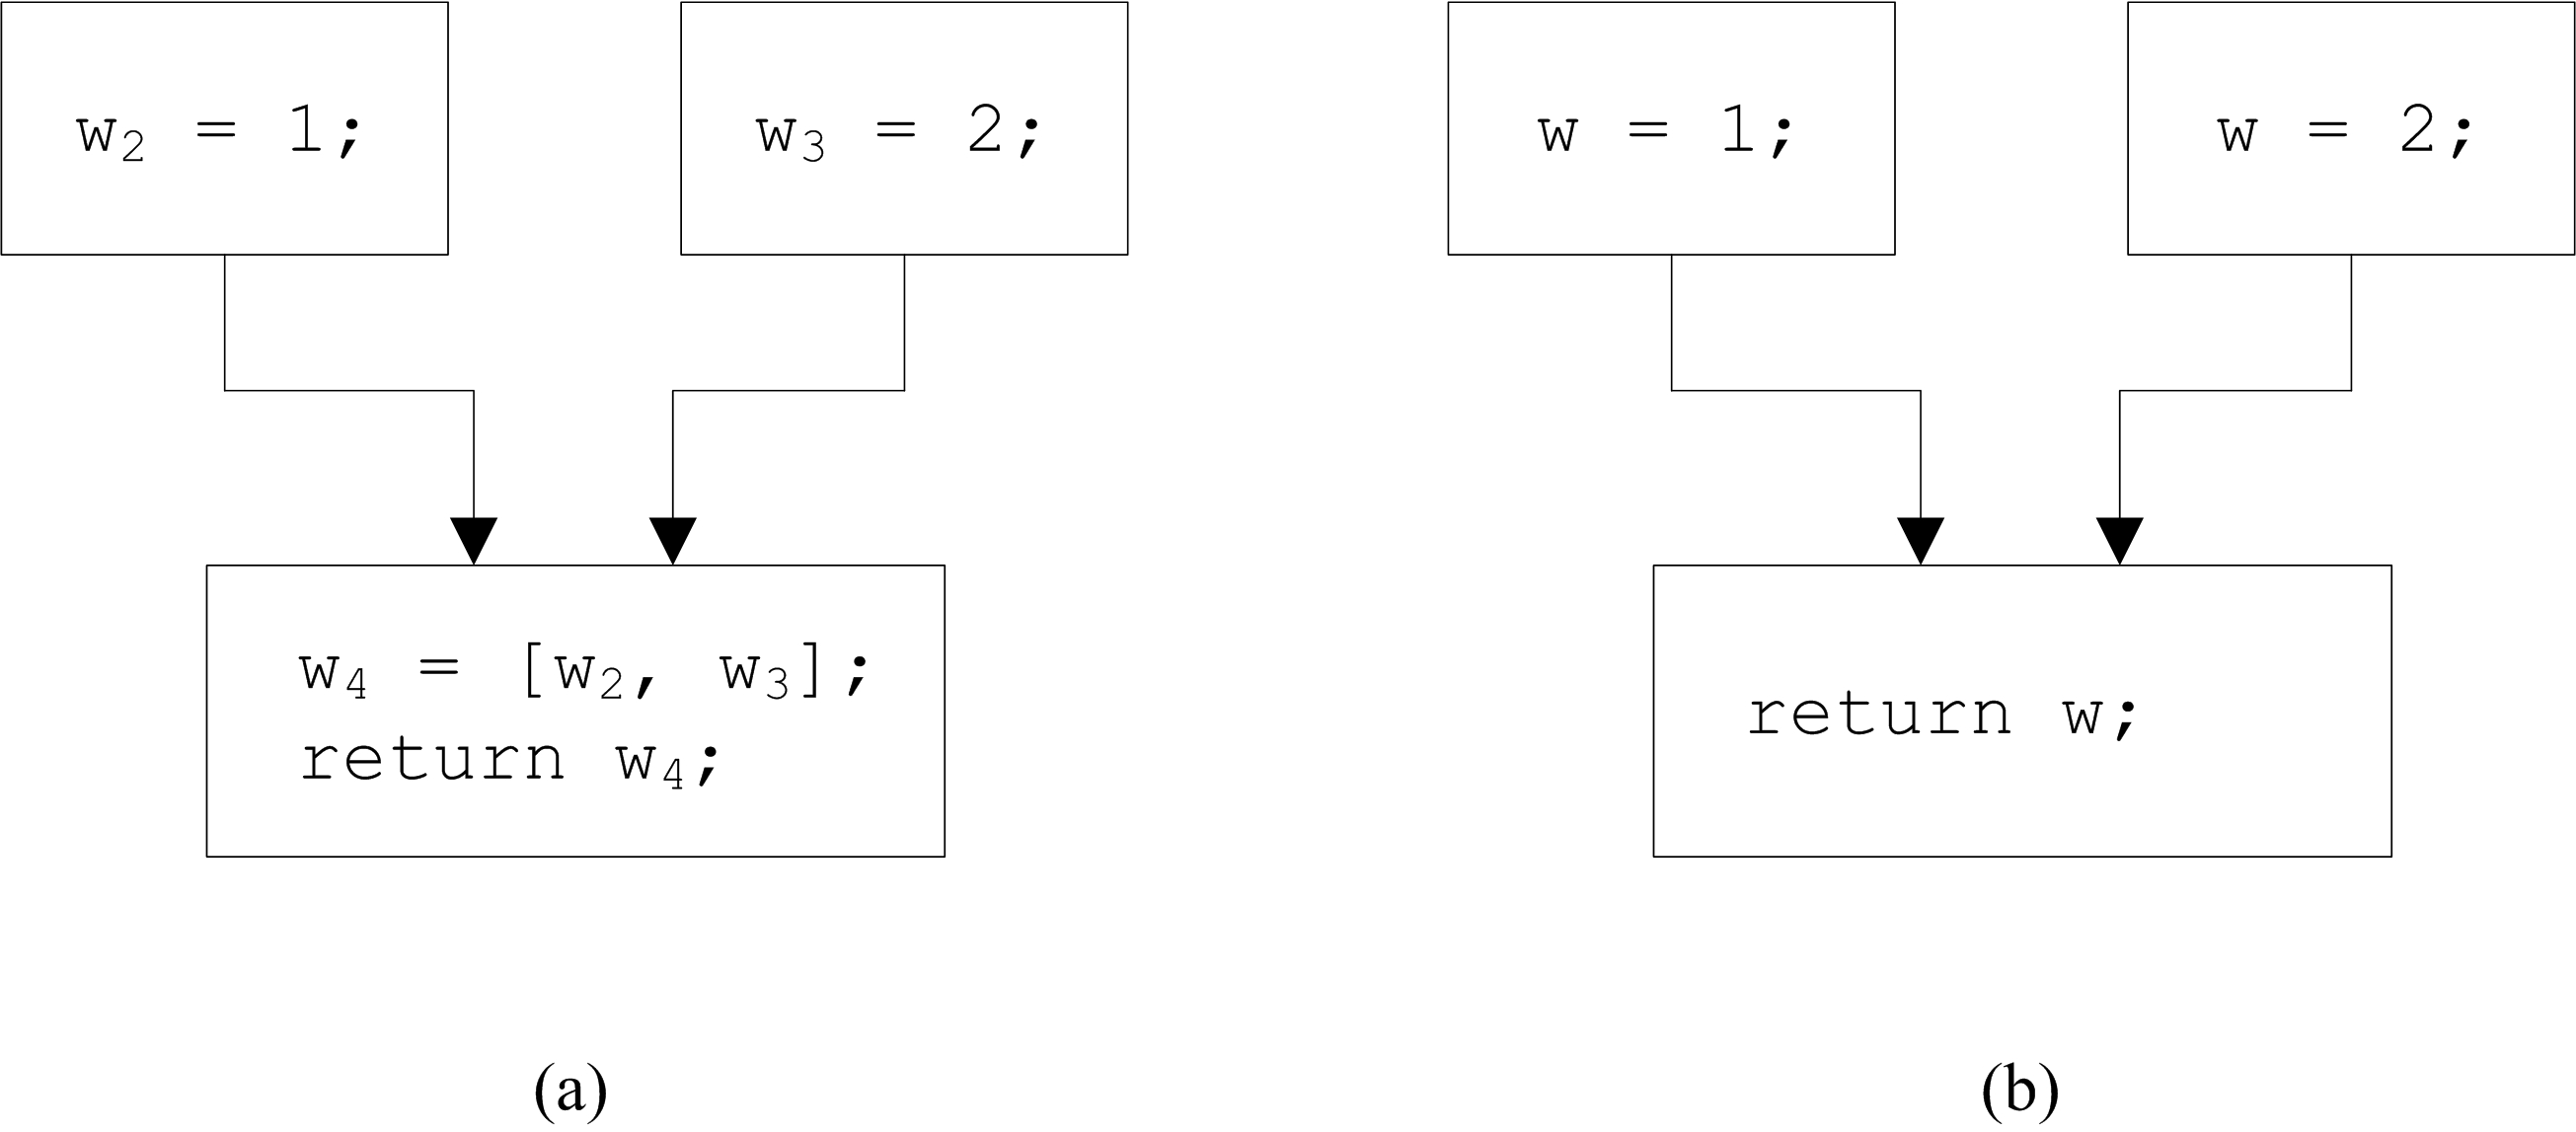
\includegraphics[scale=0.6]{{figures/figure06.12}.jpg}}
\end{center}
\end{enumerate}
\end{frame}

\begin{frame}[fragile]
\pause

A run-time environment supporting code produced for Java would require
\begin{enumerate}
\item A naming convention
\item A run-time stack
\item A representation for arrays and objects
\item A heap
\item A run-time library of code that supports the Java API
\end{enumerate}

\pause
\bigskip

We use a simple naming mechanism that takes account of just classes and their members

\pause
\bigskip

Methods are represented in SPIM by routines with assembly language names of the form \lstinline{<class>.<name>} where \lstinline{<name>} names a method in a class \lstinline{<class>}

\pause
\bigskip

Static fields are similarly named

\pause
\bigskip

String literals in the data segment have labels that suggest what they label
\end{frame}

\begin{frame}[fragile]
\pause

Our run-time stack conforms to the run-time convention described for SPIM

\pause
\bigskip

Each time a method is invoked, a new stack frame of the type shown below is pushed onto the stack; upon return from the method, the same frame is popped off from the stack
\begin{center}
\visible<3->{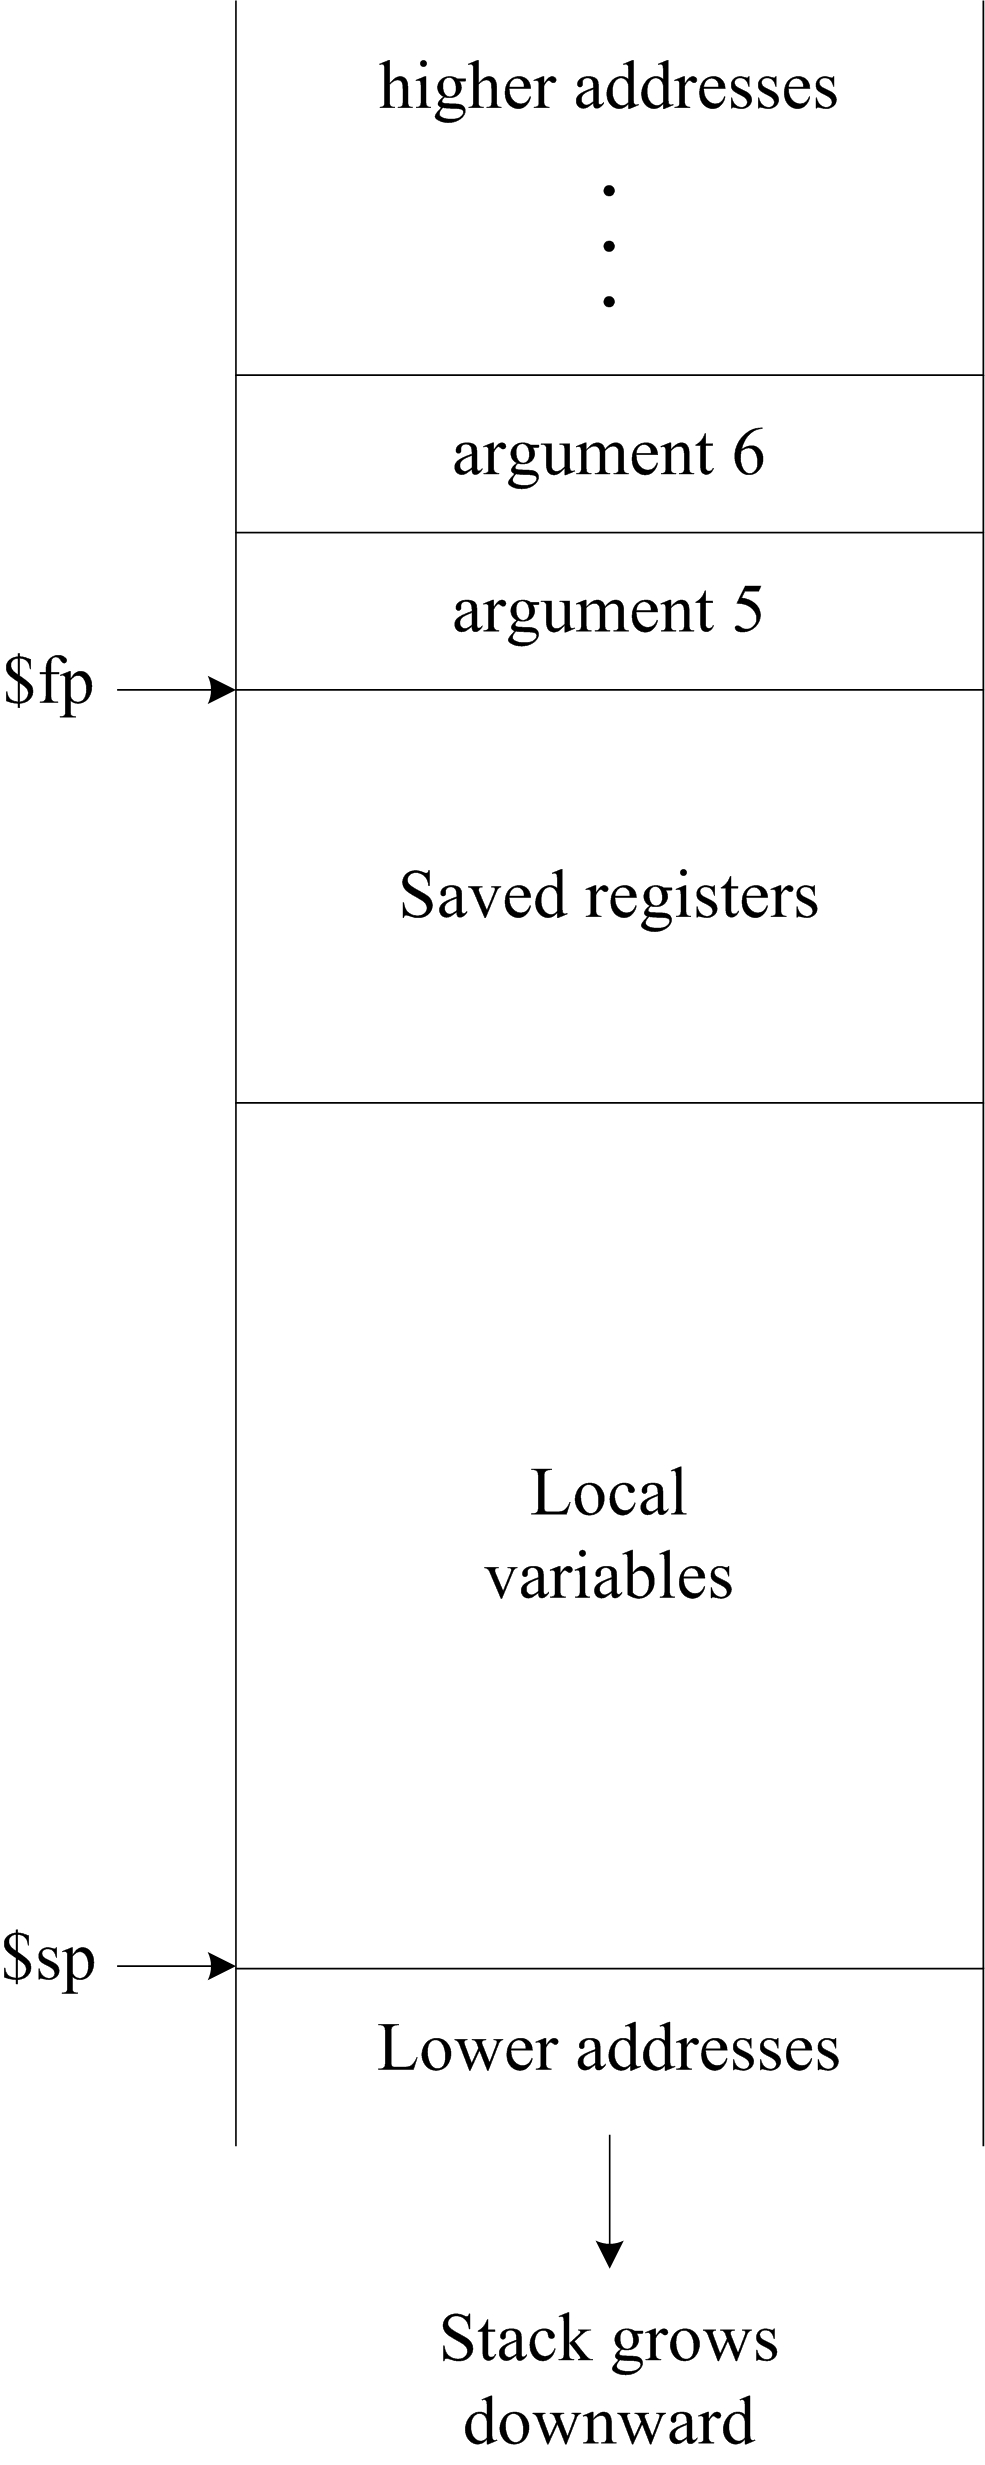
\includegraphics[scale=0.4]{{figures/figure06.04}.jpg}}
\end{center}
\end{frame}

\begin{frame}[fragile]
\pause

An arbitrary object might be organized as follows
\begin{center}
\visible<2->{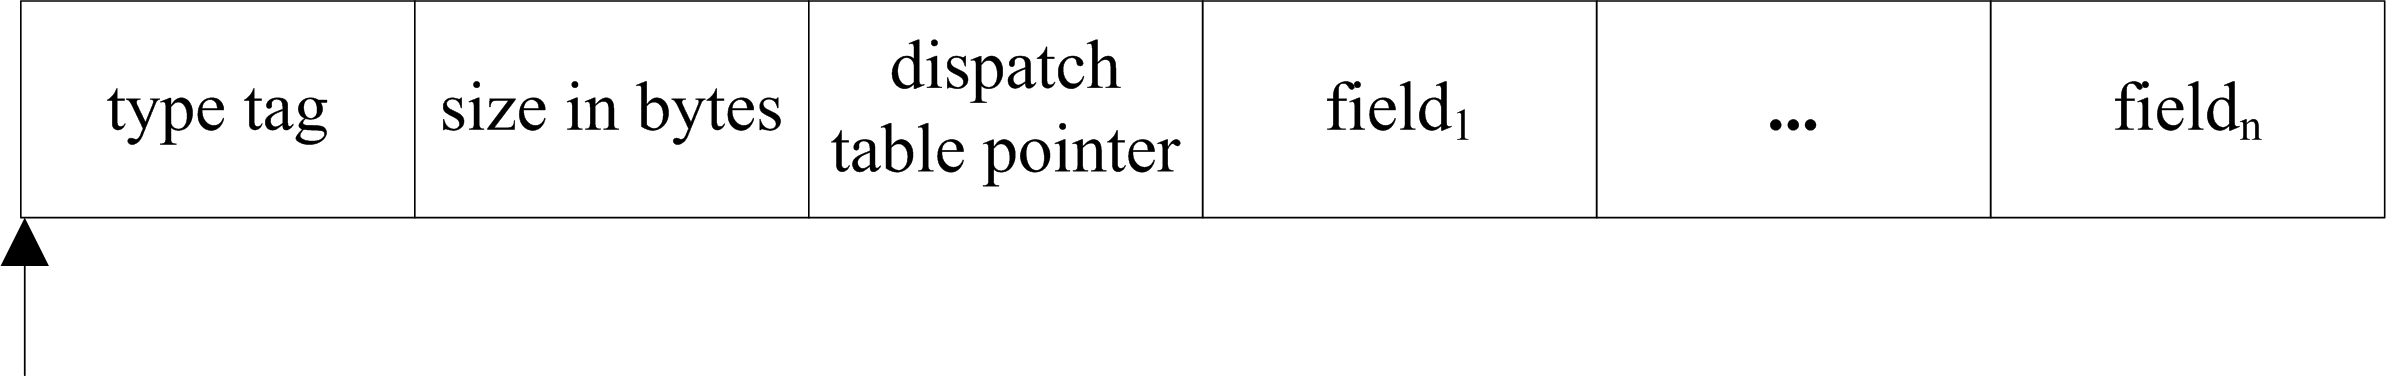
\includegraphics[scale=0.6]{{figures/figure06.14}.jpg}}
\end{center}

\pause
\bigskip

For each class, we also maintain a class template in the data segment, which among other things may include a typical copy of an object of that class that can be copied to the heap during allocation

\pause
\bigskip

For example, consider the following \jmm code
\begin{lstlisting}[language=Java]
public class Foo {
    int field1 = 1;
    int field2 = 2;

    int f() { return field1 + field2; }

    int foo() { return field1; }
}

class Bar extends Foo {
    int field3 = 3;
    int field1 = 4;

    int f() { return field1 + field2 + field3; }

    int bar() { return field1; }
}
\end{lstlisting}
\end{frame}

\begin{frame}[fragile]
\pause

Layout and dispatch table for \lstinline{Foo}
\begin{center}
\visible<2->{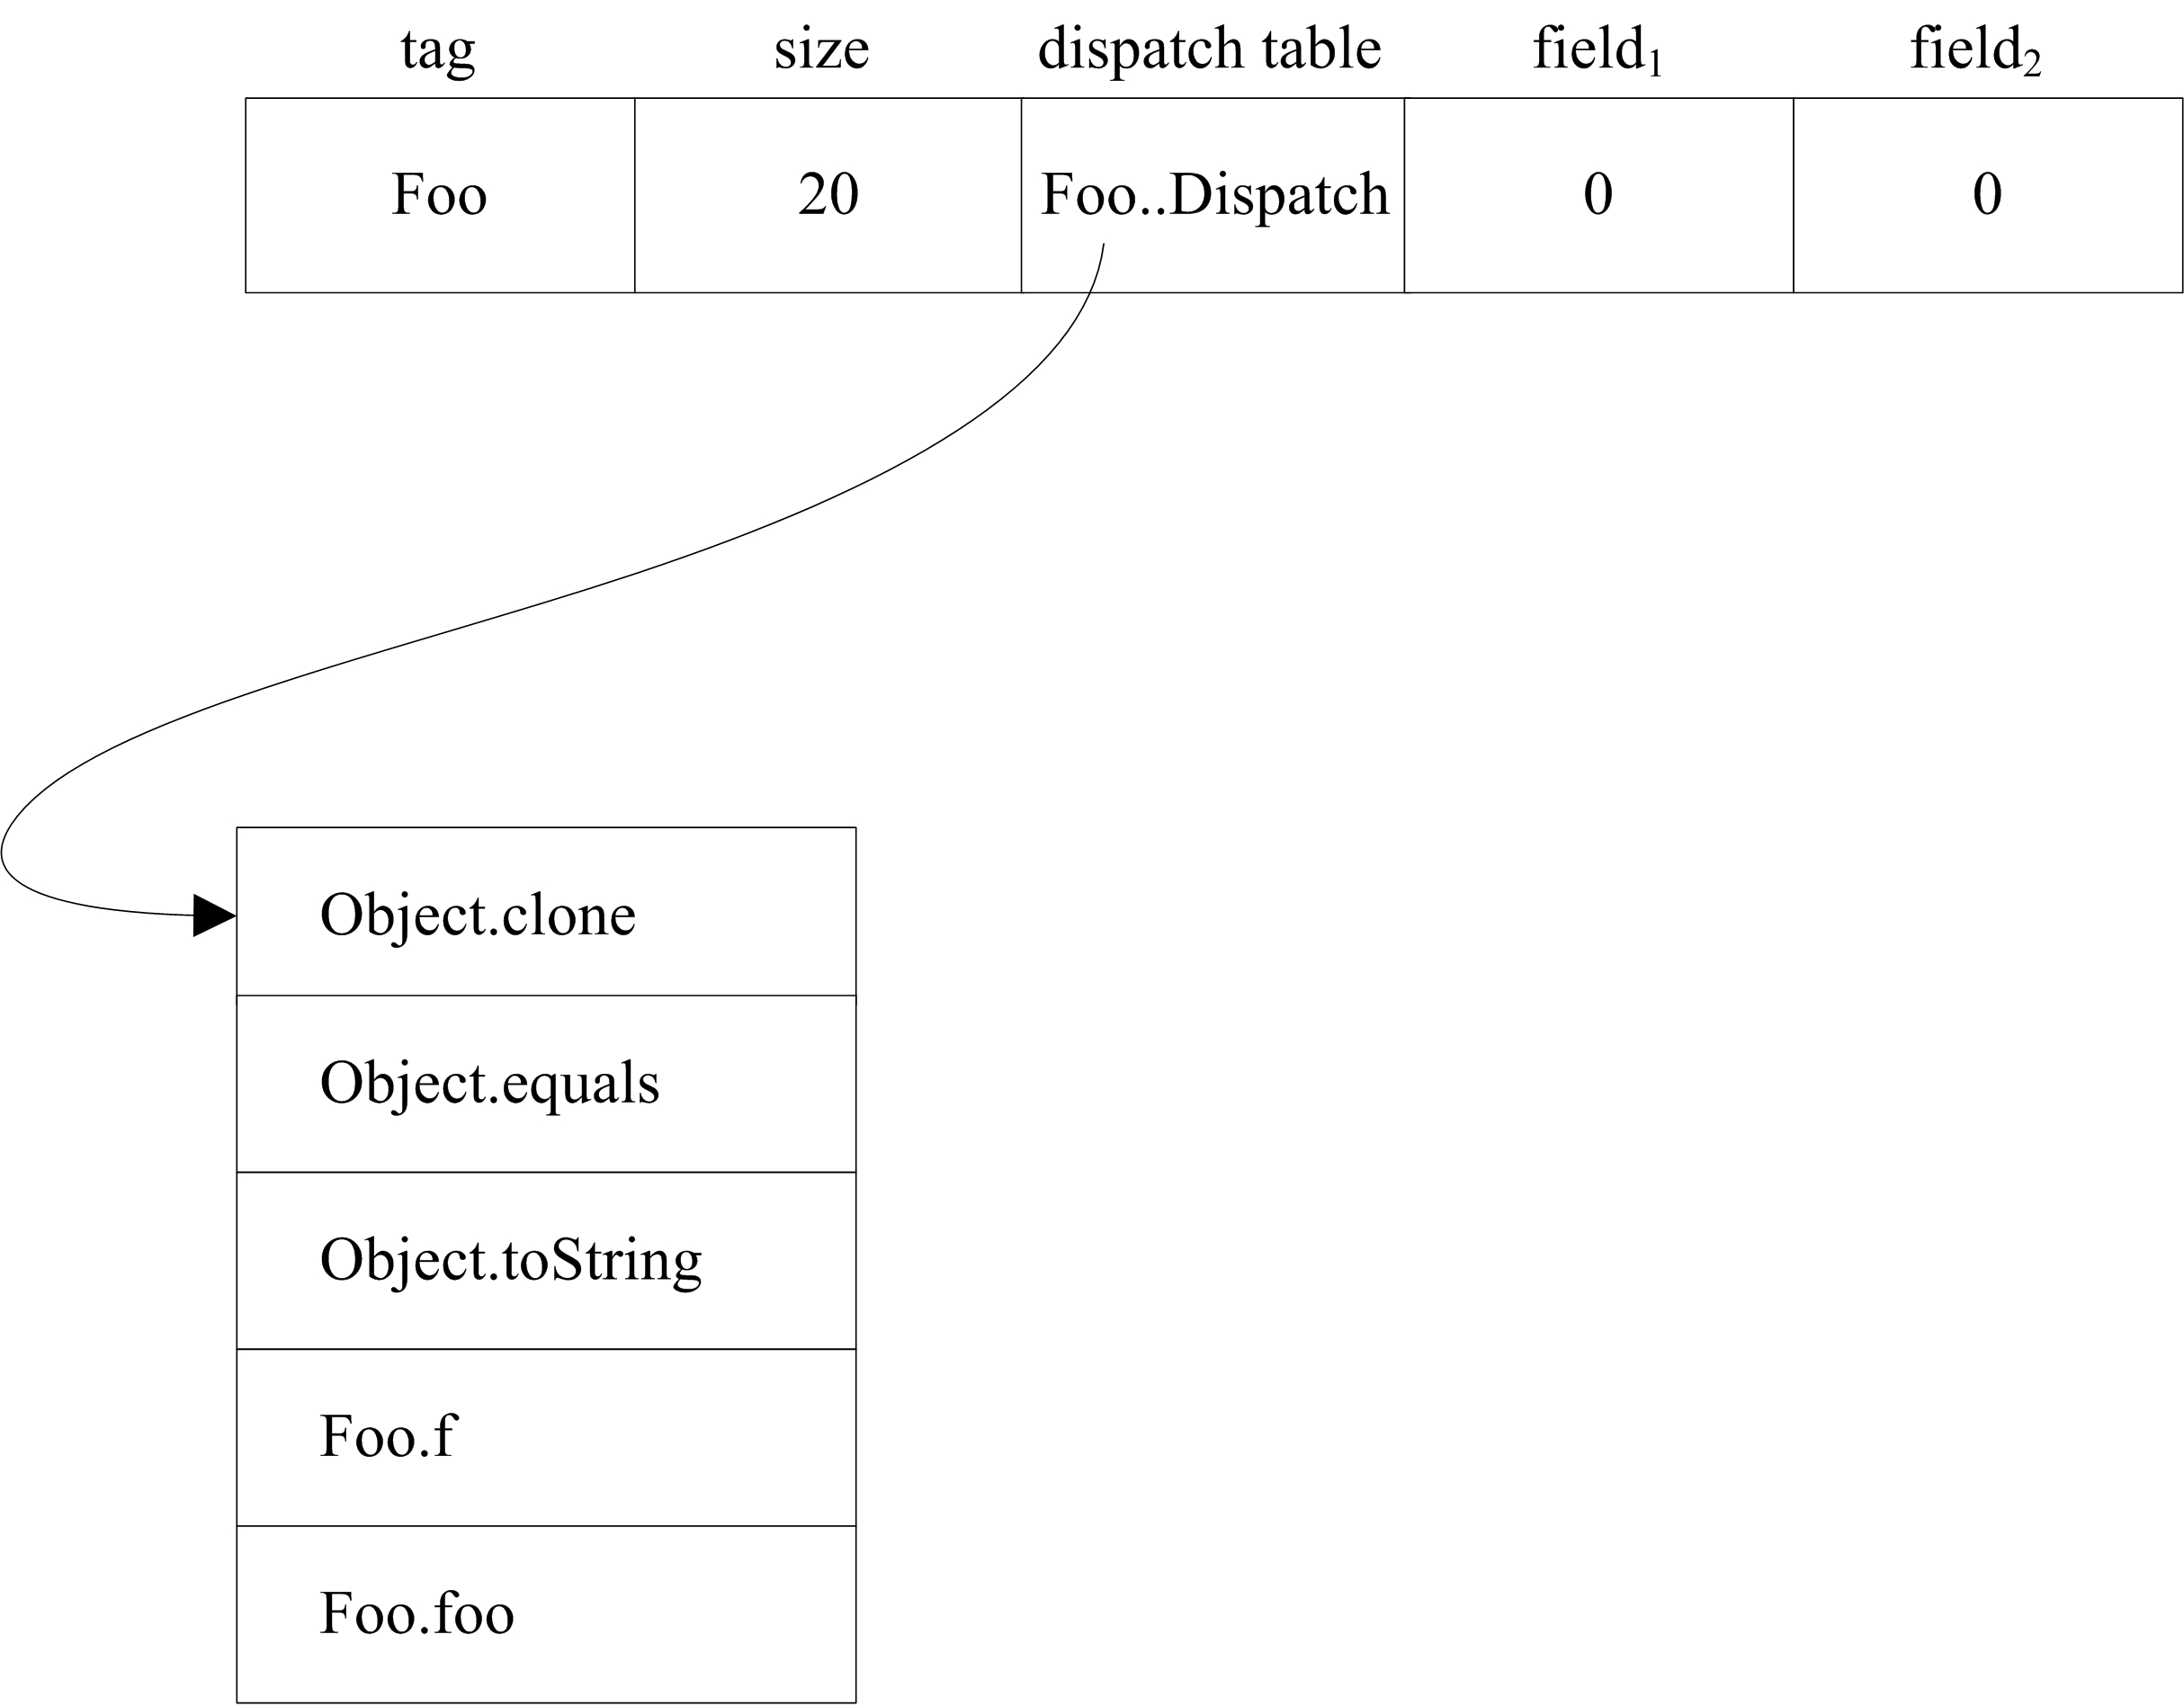
\includegraphics[scale=0.6]{{figures/figure06.15}.jpg}}
\end{center}
\end{frame}

\begin{frame}[fragile]
\pause

Layout and dispatch table for \lstinline{Bar}
\begin{center}
\visible<2->{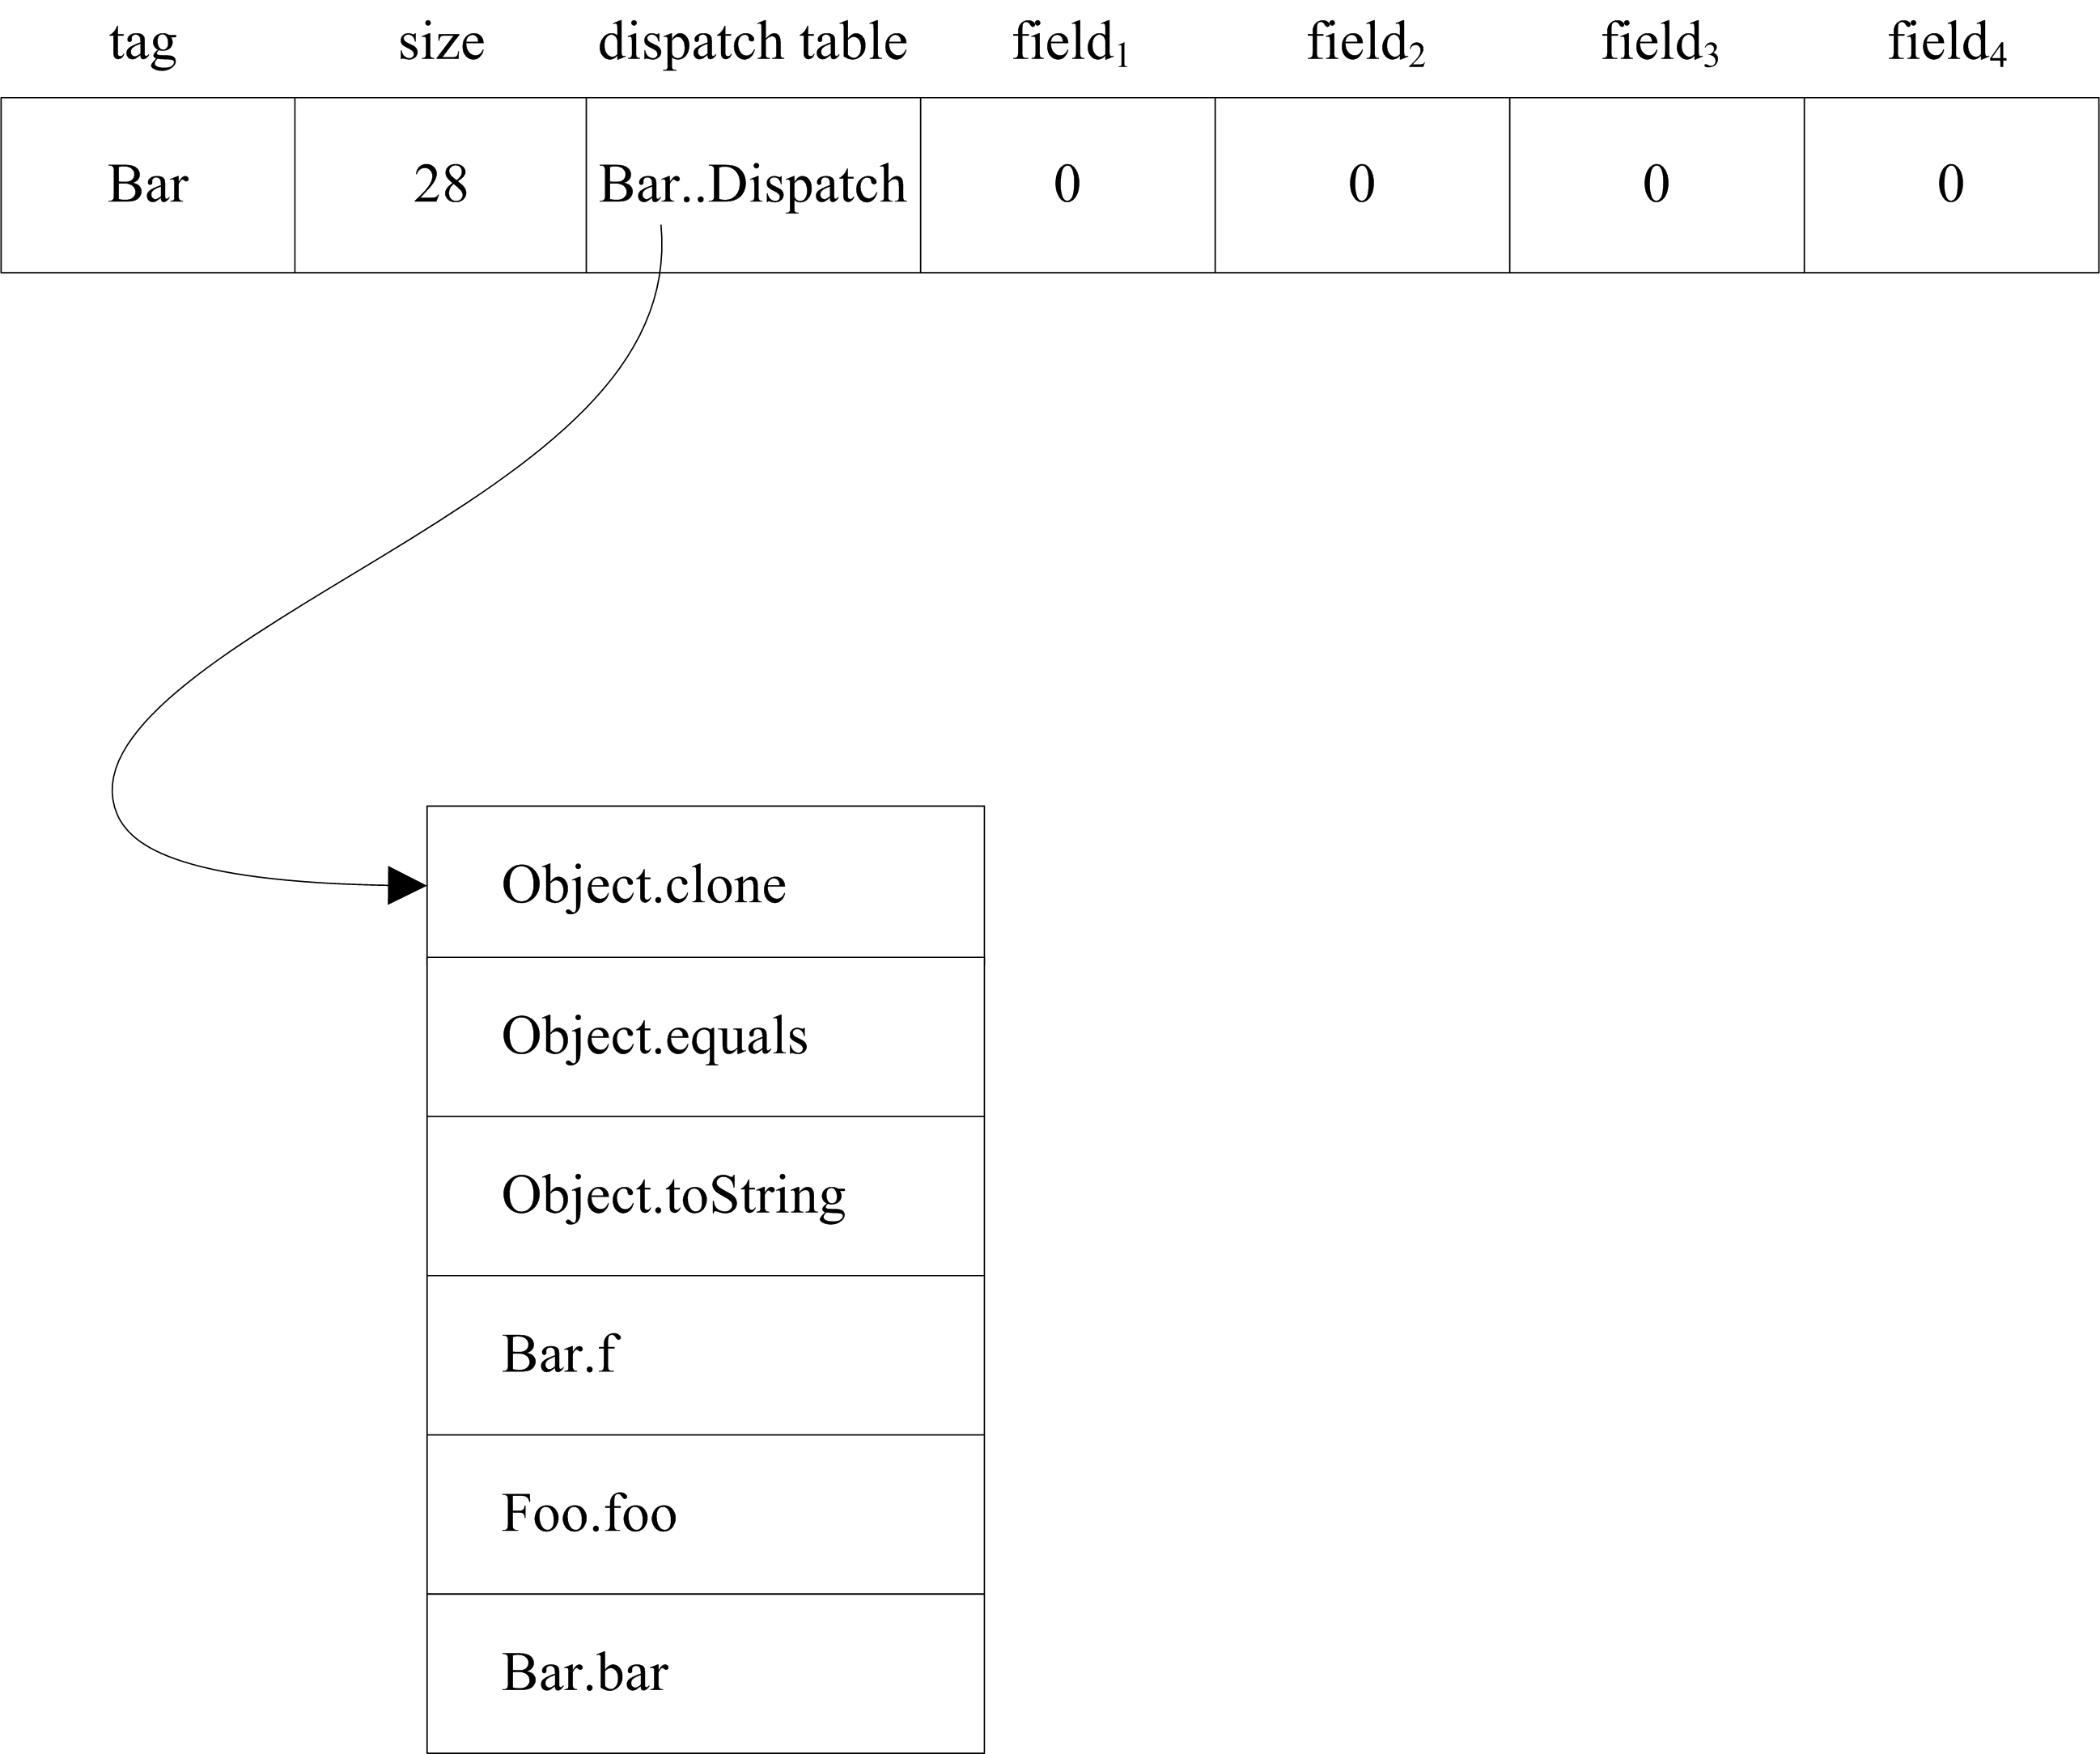
\includegraphics[scale=0.6]{{figures/figure06.16}.jpg}}
\end{center}
\end{frame}

\begin{frame}[fragile]
\pause

Arrays are a special kind of object; they are dynamically allocated on the heap but lie
outside of the \lstinline{Object} hierarchy

\pause
\bigskip

A possible layout for an array is shown below
\begin{center}
\visible<3->{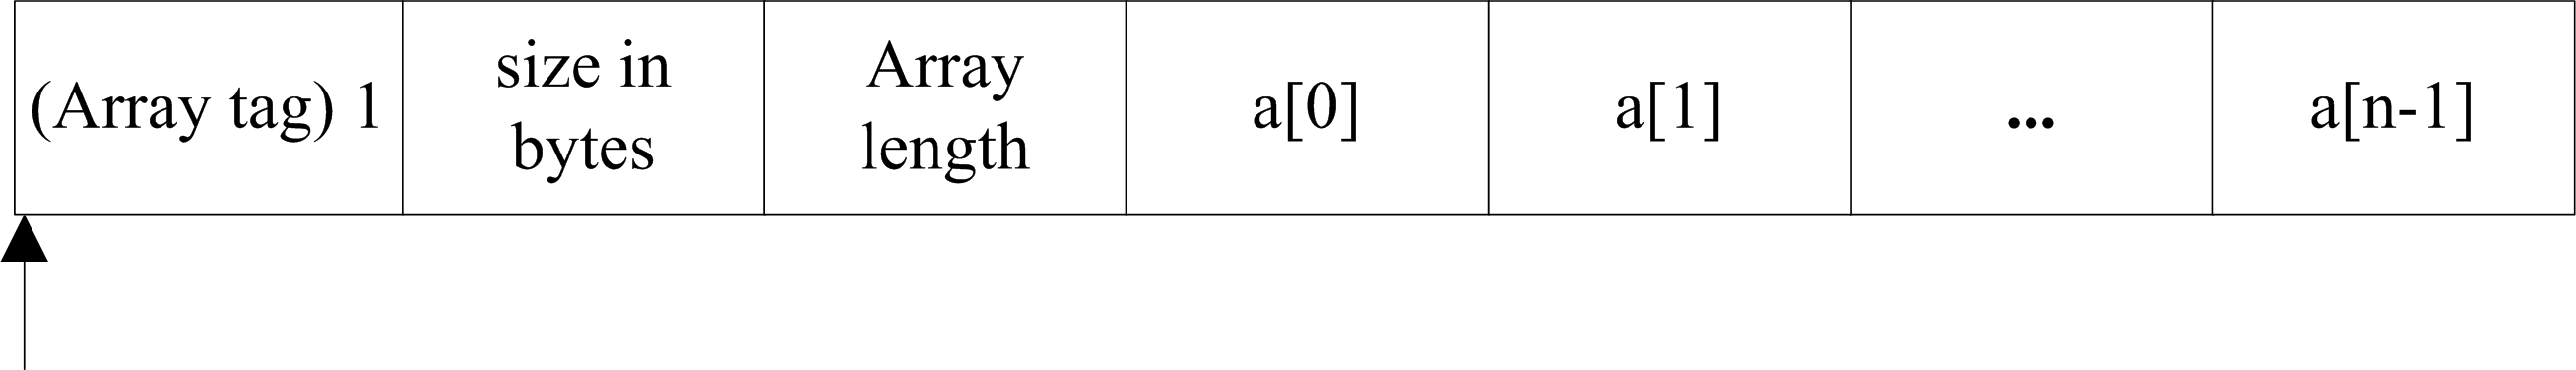
\includegraphics[scale=0.6]{{figures/figure06.17}.jpg}}
\end{center}

\pause
\bigskip

Strings are also special objects; while they are part of the \lstinline{Object} hierarchy they are
final and so they may not be sub-classed

\pause
\bigskip

A possible layout for a string is shown below
\begin{center}
\visible<5->{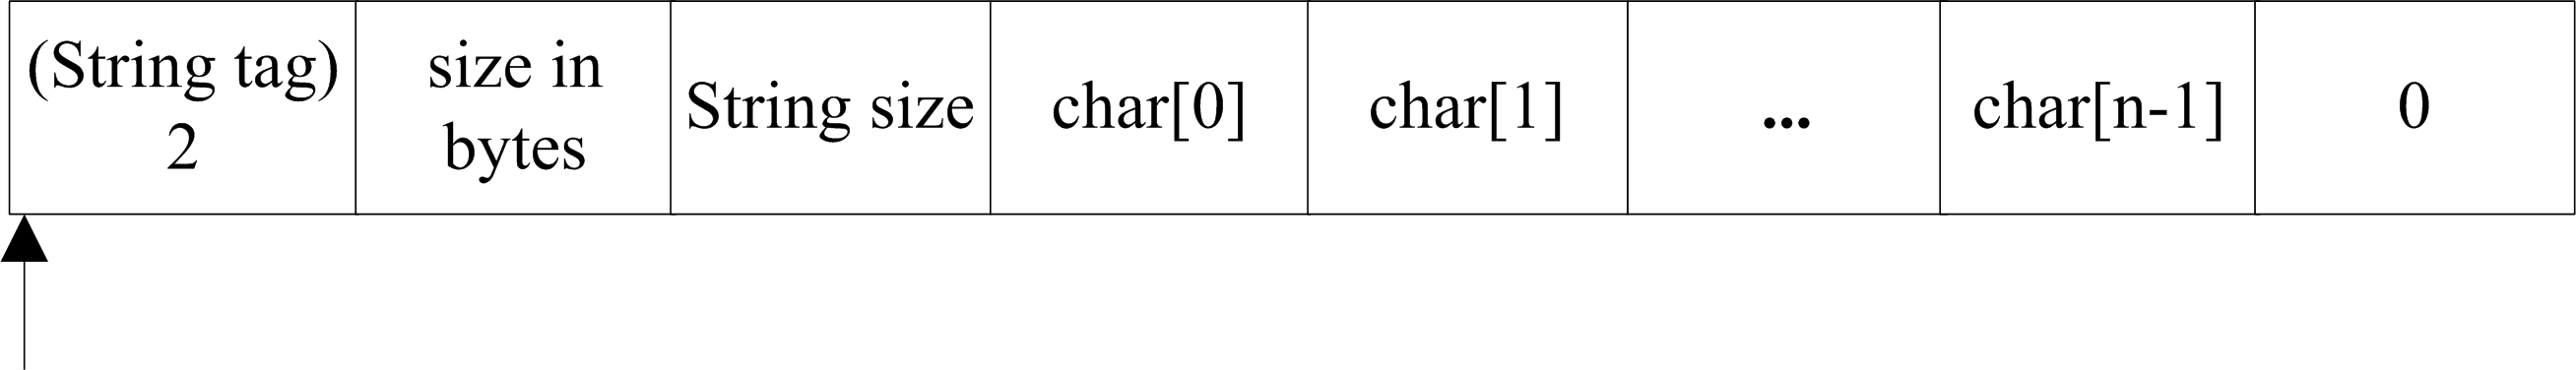
\includegraphics[scale=0.6]{{figures/figure06.18}.jpg}}
\end{center}

\pause
\bigskip

Constant strings may be allocated in the data segment, ie, we may generate constant strings in the data segment; strings in the data segment will then look exactly like those on the heap
\end{frame}

\begin{frame}[fragile]
\pause

The logic for allocating free space on the heap is pretty simple in our (oversimplified) model

\begin{lstlisting}[language={}]
obj = heapPointer;
heapPointer += <object size>;
if (heapPointer >= stackPointer) goto freakOut;
<copy object template to obj>;
\end{lstlisting}

\pause
\bigskip

When allocating a new object, we simply increment a free pointer by the appropriate size and if we've run out of space (ie, when the heap pointer meets the stack pointer), we freak out; a more robust heap management system might perform garbage collection

\pause
\bigskip

Once we have allocated the space for the object, we copy its template onto the heap at the object's location; proper initialization is left to the SPIM routines that model the constructors
\end{frame}

\begin{frame}[fragile]
\pause

SPIM provides a set of built-in system calls for performing simple I/O tasks

\pause
\bigskip

Our runtime environment includes a class \lstinline{SPIM}, which is a wrapper that gives us access to these calls as a set of static methods

\begin{lstlisting}[language=Java]
package spim;

public class SPIM {
    public static void printInt(int value) { }
    public static void printFloat(float value) { }
    public static void printDouble(double value) { }
    public static void printString(String value) { }
    public static void printChar(char value) { }
    public static int readInt() { return 0; }
    public static float readFloat() { return 0; }
    public static double readDouble() { return 0; }
    public static String readString(int length) { return null; }
    public static char readChar() { return ' '; }
    public static int open(String filename, int flags, int mode) { return 0; }
    public static String read(int fd, int length) { return null; }
    public static int write(int fd, String buffer, int length) { return 0; }
    public static void close(int fd) { }
    public static void exit() { }
    public static void exit2(int status) { }
}
\end{lstlisting}

\pause
\bigskip

Since the \lstinline{SPIM} class is defined in the package \lstinline{spim}, that package name is part of the label for the entry point to each SPIM method; for example
\begin{lstlisting}[language={}]
spim.SPIM.printInt:
\end{lstlisting}
\end{frame}

\begin{frame}[fragile]
\pause

Once virtual registers have been mapped to physical registers, translating LIR to SPIM code is pretty straightforward

\pause
\bigskip

We iterate through the list of methods for each class; for each method, we do the following
\begin{itemize}
\item We generate a label for the method's entry point

\item We generate code to push a new frame onto the run-time stack and then code to save all our registers; we treat all of SPIM's general purpose registers \$t0 -- \$t9 and \$s0 -- \$s7 as callee-saved registers

\item Since all branches in the code are expressed as branches to basic blocks, a unique label for each basic block is generated into the code

\item We then iterate through the LIR instructions for the block, invoking a method \lstinline{toSpim()}, which is defined for each LIR instruction; there is a one-to-one translation from each LIR instruction to its SPIM equivalent

\item Any string literals that are encountered in the instructions are put into a list, together with appropriate labels; these will be emitted into a data segment at the end of the method

\item We generate code to restore those registers that had been saved at the start; this code also does a jump to that instruction following the call in the calling code, which had been stored in the \$ra register
\end{itemize}
\end{frame}

\begin{frame}[fragile]
\pause

After we have generated the text portion (the program instructions) for the method, we then populate
a data area from the list of string literals constructed previously; any other literals that you may wish to implement would be handled in the same way

\pause
\bigskip

Once all of the program code has been generated, we then copy out the SPIM code for implementing the \lstinline{SPIM} class

\pause
\bigskip

For example, the SPIM code for \lstinline{Factorial.computeIter()} is as follows
\begin{lstlisting}[language={}]
.text

Factorial.computeIter:
    subu    $sp,$sp,36   # Stack frame is 36 bytes long
    sw      $ra,32($sp)  # Save return address
    sw      $fp,28($sp)  # Save frame pointer
    sw      $t0,24($sp)  # Save register $t0                                                                                                                                                                                                  
    sw      $t1,20($sp)  # Save register $t1
    sw      $t2,16($sp)  # Save register $t2                                                                                                                                                                                                  
    sw      $t3,12($sp)  # Save register $t3
    sw      $t4,8($sp)   # Save register $t4                                                                                                                                                                                                  
    sw      $t5,4($sp)   # Save register $t5
    sw      $t6,0($sp)   # Save register $t6                                                                                                                                                                                                  
    addiu   $fp,$sp,32   # Save frame pointer                                                                                                                                                                                                 
                                                                                                                                                                                                                                              
Factorial.computeIter.0:                                                                                                                                                                                                                      
                                                                                                                                                                                                                                              
Factorial.computeIter.1:                                                                                                                                                                                                                      
    li $t0,1
    move $t1,$a0
    move $t2,$t0
\end{lstlisting}
\end{frame}

\begin{frame}[fragile]
\pause

\begin{lstlisting}[language={}]
Factorial.computeIter.2:
    li $t3,0                                                                                                                                                                                                                                  
    ble $t1,$t3,Factorial.computeIter.4
    j Factorial.computeIter.3

Factorial.computeIter.3:
    li $t4,-1                                                                                                                                                                                                                                 
    add $t5,$t1,$t4
    mul $t6,$t2,$t1                                                                                                                                                                                                                           
    move $t2,$t6                                                                                                                                                                                                                              
    move $t1,$t5                                                                                                                                                                                                                              
    j Factorial.computeIter.2                                                                                                                                                                                                                 
                                                                                                                                                                                                                                              
Factorial.computeIter.4:                                                                                                                                                                                                                      
    move $v0,$t2                                                                                                                                                                                                                              
    j Factorial.computeIter.restore                                                                                                                                                                                                           
                                                                                                                                                                                                                                              
Factorial.computeIter.restore:                                                                                                                                                                                                                
    lw      $ra,32($sp)  # Restore return address                                                                                                                                                                                             
    lw      $fp,28($sp)  # Restore frame pointer                                                                                                                                                                                              
    lw      $t0,24($sp)  # Restore register $t0
    lw      $t1,20($sp)  # Restore register $t1                                                                                                                                                                                               
    lw      $t2,16($sp)  # Restore register $t2
    lw      $t3,12($sp)  # Restore register $t3                                                                                                                                                                                               
    lw      $t4,8($sp)   # Restore register $t4
    lw      $t5,4($sp)   # Restore register $t5                                                                                                                                                                                               
    lw      $t6,0($sp)   # Restore register $t6
    addiu   $sp,$sp,36   # Pop stack
    jr      $ra          # Return to caller
\end{lstlisting}

\pause
\bigskip

We can perform peephole optimizations (considering just a few instuctions at a time) on the SPIM code to remove jumps to immediate instructions and simplify jumps to jumps
\end{frame}
\end{document}
